\documentclass[11pt,letterpaper]{article}
\usepackage[margin=0.85in,headheight=14pt]{geometry}
\usepackage{lmodern,amsmath,amssymb,amsthm,booktabs,array,longtable,graphicx,lscape,float}
\usepackage{fancyhdr}
\usepackage{color}
\definecolor{linkblue}{rgb}{0.1,0.2,0.35}
\usepackage[colorlinks=true,linkcolor=linkblue,citecolor=linkblue,urlcolor=linkblue]{hyperref}
\pagestyle{fancy}
\fancyhf{}
\fancyhead[L]{\small Synthetic tabular data on known distributions}
\fancyhead[R]{\small Experimental report}
\fancyfoot[C]{\thepage}
\setlength{\parskip}{0.2em}
\setlength{\tabcolsep}{5pt}
\renewcommand{\arraystretch}{1.08}
\newcommand{\E}{\mathbb{E}}
\newcommand{\Prb}{\mathbb{P}}
\newcommand{\ind}{\mathbf{1}}
\newcommand{\KL}{D_{\mathrm{KL}}}
\newcommand{\Lsyn}{L_{\mathrm{syn}}}
\newcommand{\Ltest}{L_{\mathrm{test}}}
\newcommand{\Normal}{\mathcal{N}}
\newtheorem{proposition}{Proposition}
\title{Likelihood and Predictive Utility of Synthetic Tabular Data:\\CTGAN and TVAE on Known Distributions}
\author{}
\date{1 October 2026}
\begin{document}
\maketitle
\begin{abstract}
We evaluate CTGAN and TVAE on four established Bayesian networks and three mixed-data distributions with an analytically specified classification target. The mixed benchmarks isolate independent Gaussian features, independent multimodal features, and dependent multimodal features while retaining a common categorical mechanism and target noise model. Each dataset is evaluated with original-data training, complete-table synthesis, and six supervised relabelers applied to either jointly generated or separately generated features. The experiment contains 378 dataset--seed--method evaluations. Evaluation combines original-model likelihood, likelihood under a synthetic-data refit, test accuracy, macro F1, and agreement with the exact Bayes classifier. Bayesian-network likelihoods use the historical SDGym adjustment $\log(p+10^{-8})$. Relabeling frequently recovers the prediction performance of original-data training without recovering its joint-distribution score. For example, CTGAN--joint--XGB attains 95.06\% accuracy on Insurance, while 48.33\% of its rows have zero probability under the original network. We derive the Bayes accuracy and the relationship between noisy-target accuracy and oracle agreement, and compare the results with the original CTGAN paper and its supplement.
\end{abstract}

\section{Scope and experimental design}
Xu et al.~\cite{xu2019} evaluate synthetic data through two likelihood directions on simulated data and through downstream prediction on real data. We retain both likelihood directions and extend the simulated setting with explicit prediction tasks. Four datasets, Asia, Alarm, Child, and Insurance, retain their Bayesian-network joint distributions. Three further datasets, Gaussian, Grid, and Ring, use a common mixed-data construction with a known decision boundary. The new Grid and Ring tasks differ from the original paper's two-column Gaussian-mixture datasets. Their scores are therefore reported as additional results, separately from the archived reproduction of the original mixture benchmark.

For each dataset and seed $s\in\{42,43\}$, the original distribution $P$ supplies independent training and test tables of 10,000 rows each. Each synthesizer produces 10,000 rows. Every method within a dataset--seed pair uses the same original test table. We fit all supervised relabelers on the original training table and train a fresh evaluation classifier on the resulting labeled table. All reported current-run means are arithmetic averages over the two seeds. Seed dispersion is displayed in the figures; it is not a confidence interval.

\section{Data-generating distributions}
\subsection{Mixed-data construction}
Write a row as $Z=(X_0,X_1,C,Y)$, where $C$ is the column \texttt{feature\_3} and $Y$ is \texttt{target}. The feature vector used for prediction is $W=(X_0,X_1,C)$. Let $\sigma(t)=(1+e^{-t})^{-1}$. For all three mixed datasets,
\begin{align}
 C\mid X_0=x_0,X_1=x_1 &\sim \operatorname{Bernoulli}(a(x)),
 &a(x)&=\sigma(\kappa x_0x_1), \label{eq:category}\\
 h^*(x,c)&=\ind\{x_1+[1+\beta(2c-1)]x_0>0\}, \label{eq:boundary}\\
 E&\sim\operatorname{Bernoulli}(\eta),\quad E\perp(X_0,X_1,C),
 &Y&=h^*(X,C)\mathbin{\oplus} E. \label{eq:noise}
\end{align}
Here $\oplus$ denotes exclusive OR. We use $\kappa=2$, $\beta=0.75$, and $\eta=0.10$. Changing $C$ changes the coefficient of $X_0$ from 0.25 to 1.75. The normalized joint density, relative to Lebesgue measure on $\mathbb{R}^2$ and counting measure on $\{0,1\}^2$, is
\begin{equation}
 p(x,c,y)=f_X(x)\,a(x)^c[1-a(x)]^{1-c}
 (1-\eta)^{\ind\{y=h^*(x,c)\}}\eta^{\ind\{y\ne h^*(x,c)\}}.
 \label{eq:mixedjoint}
\end{equation}
Only $f_X$ changes between datasets. Feature scaling uses known population moments, not estimated moments from a training or test table.

\paragraph{Gaussian.} The continuous features are independent standard normals:
\begin{equation}
 X_0,X_1\stackrel{\mathrm{iid}}{\sim}\Normal(0,1),\qquad
 f_X(x)=\phi(x_0)\phi(x_1).
\end{equation}

\paragraph{Grid.} Let $A=\{-4,-2,0,2,4\}$, $M_0,M_1\stackrel{\mathrm{iid}}{\sim}\operatorname{Unif}(A)$, and $U_0,U_1\stackrel{\mathrm{iid}}{\sim}\Normal(0,1)$, mutually independent. With $\tau=0.20$ and $s_G=\sqrt{8+\tau^2}$, set
\begin{equation}
 X_j=\frac{M_j+\tau U_j}{s_G},\qquad
 f_X(x)=\prod_{j=0}^{1}\left[\frac15\sum_{m\in A}
 \phi\left(x_j;\frac{m}{s_G},\frac{\tau^2}{s_G^2}\right)\right].
 \label{eq:grid}
\end{equation}
Here $\phi(\cdot;\mu,v)$ denotes a normal density with variance $v$. The resulting distribution has 25 equally weighted joint components and independent coordinates.

\paragraph{Ring.} Let $K\sim\operatorname{Unif}\{0,\ldots,7\}$, $\theta_k=k\pi/4$, $\mu_k=(\cos\theta_k,\sin\theta_k)$, and $U\sim\Normal(0,I_2)$ independent of $K$. With $s_R=\sqrt{1/2+\tau^2}$, set
\begin{equation}
 X=\frac{\mu_K+\tau U}{s_R},\qquad
 f_X(x)=\frac18\sum_{k=0}^{7}
 \phi_2\left(x;\frac{\mu_k}{s_R},\frac{\tau^2}{s_R^2}I_2\right).
 \label{eq:ring}
\end{equation}
The same latent component selects both coordinates. Ring tests dependence that is absent from Gaussian and Grid.

\begin{proposition}[Feature and target structure]
In all three mixed datasets, each continuous coordinate has mean zero and variance one. Gaussian and Grid have independent coordinates. Ring has zero covariance but dependent coordinates. Furthermore, $\Prb(C=1\mid X_j)=1/2$ for $j=0,1$, and both $h^*(W)$ and $Y$ are marginally balanced.
\end{proposition}
\begin{proof}
The Gaussian statement is immediate. For Grid, $\E M_j=0$ and $\E M_j^2=8$; independence follows from independent coordinate-specific component and noise draws. For Ring, $\E\mu_K=0$, $\E\mu_K\mu_K^\top=I_2/2$, and the stated scale gives identity covariance. Dependence follows from
\[
 \E[X_0^2X_1^2]=\frac{1/8+\tau^2+\tau^4}{(1/2+\tau^2)^2}<1
 =\E[X_0^2]\E[X_1^2].
\]
Each feature distribution is invariant to reflection of either coordinate. Conditional reflection symmetry and $\sigma(t)+\sigma(-t)=1$ give the category marginal. Simultaneous negation of $X_0,X_1$ preserves $a(x)$ and reverses the score in~\eqref{eq:boundary}. Its zero set has probability zero. Hence $h^*$ is balanced, and independent symmetric label flips preserve that balance.
\end{proof}

\subsection{Bayesian-network construction}
Let $V=(V_1,\ldots,V_d)$ follow a directed acyclic graph $\mathcal{G}$ with the packaged BIF conditional probability tables. The joint mass function is
\begin{equation}
 p(v)=\prod_{j=1}^{d}p_j(v_j\mid v_{\operatorname{pa}(j)}).
 \label{eq:bnjoint}
\end{equation}
Rows are sampled ancestrally in topological order. The original conditional tables, including exact zero probabilities, are retained. There is no added target noise. Table~\ref{tab:bntasks} specifies the target; all remaining nodes are observed features. Integer codes identify categorical states and have no ordinal interpretation.
\begin{table}[H]\centering
\caption{Bayesian-network prediction tasks. Cardinality counts the target's possible states.}\label{tab:bntasks}
\begin{tabular}{lrrlr}\toprule
Dataset & Nodes & Features & Target node & Cardinality\\\midrule
Asia & 8 & 7 & \texttt{dysp} & 2\\
Alarm & 37 & 36 & \texttt{BP} & 3\\
Child & 20 & 19 & \texttt{Disease} & 6\\
Insurance & 27 & 26 & \texttt{Accident} & 4\\\bottomrule
\end{tabular}
\end{table}
For an original-distribution feature vector $w$, the exact posterior and Bayes decision are
\begin{equation}
 \pi_y(w)=\Prb(Y=y\mid W=w)=\frac{p(w,y)}{\sum_{u\in\mathcal{Y}}p(w,u)},
 \qquad h^*(w)=\arg\max_{y\in\mathcal{Y}}\pi_y(w).
 \label{eq:bnposterior}
\end{equation}
Ties are resolved by the lowest state index. Evaluating all target states is exact because every other node is observed. The conditional distribution depends on the network's relevant conditional structure; no claim is made that every feature is needed for prediction.

\section{Synthesis and supervised relabeling}
CTGAN uses a conditional adversarial generator and TVAE uses a variational autoencoder~\cite{xu2019,ctganimplementation}. We use CTGAN package version 0.10.2 with 300 epochs, batch size 500, and the package's remaining defaults. A complete-table generator is fitted to $(W,Y)$; a feature-only generator is fitted separately to $W$. In the latter case, $W$ is generated by the synthesizer itself. No external sampler separates features from a fitted complete-table model.

Let $q_G(w,y)$ denote the complete-table generator distribution, $q_{G,W}(w)=\sum_y q_G(w,y)$ its feature marginal, $q_{G,F}(w)$ the separately fitted feature generator, and $a_\ell$ a relabeler trained on the original training table. The three synthetic families are
\begin{align}
 Q_{G,\mathrm{base}}(w,y)&=q_G(w,y),\\
 Q_{G,\mathrm{joint},\ell}(w,y)&=q_{G,W}(w)\ind\{y=a_\ell(w)\},\\
 Q_{G,\mathrm{features},\ell}(w,y)&=q_{G,F}(w)\ind\{y=a_\ell(w)\}.
 \label{eq:families}
\end{align}
Joint variants retain the sampled features and replace only the generated target. Feature-only variants generate $W$ with their separately trained synthesizer and then attach a target. All six labelers within each source group receive the same feature rows. Relabeling is deterministic and does not add independent label noise.

The six relabelers are Gaussian naive Bayes (GNB), categorical naive Bayes (CNB), PCA--GMM, random forest (RF), XGBoost (XGB), and a neural classifier (DNN). GNB models each encoded feature with a Gaussian within each class. CNB quantile-bins continuous features into ten bins and leaves categorical features discrete. PCA--GMM standardizes the encoded input, projects it to two principal components, and fits four full-covariance Gaussian components per observed class with empirical class priors. RF uses 100 trees. XGB uses 100 trees of maximum depth six and learning rate 0.1. Other than CNB, the labelers one-hot encode categorical inputs using the known state schema.

Every downstream evaluation uses a newly fitted DNN with two 64-unit hidden layers, standardized inputs, batch size 256, at most 100 iterations, and early stopping on an internal 10\% training split. The DNN relabeler has the same architecture but is fitted separately to original training data. RF never replaces the downstream evaluation DNN. With two generators and six labelers, there are
\begin{equation}
 1+2[1+2(6)]=27
\end{equation}
methods per dataset--seed pair: one original-data baseline, two complete-table baselines, and 24 relabeling variants. Seven datasets and two seeds give $7\times2\times27=378$ evaluations.

\section{Evaluation}
\subsection{Two likelihood directions}
Let $S=\{z_i\}_{i=1}^{N}$ be the method's training table and $T=\{z_j^{\mathrm{test}}\}_{j=1}^{M}$ the independent original test table. For the original baseline, $S$ is the original training sample. Let $\widehat q_S$ be a normalized probability model fitted using $S$ alone. Define
\begin{equation}
 g_\epsilon(t)=\log(t+\epsilon),\qquad
 \epsilon_D=\begin{cases}0,&D\in\{\text{Gaussian, Grid, Ring}\},\\10^{-8},&D\text{ is a BN dataset}.
 \end{cases}
\end{equation}
The reported likelihoods are
\begin{equation}
 \widehat\Lsyn(S)=\frac1N\sum_{i=1}^{N}g_{\epsilon_D}(p(z_i)),\qquad
 \widehat\Ltest(S,T)=\frac1M\sum_{j=1}^{M}g_{\epsilon_D}(\widehat q_S(z_j^{\mathrm{test}})).
 \label{eq:likelihoods}
\end{equation}
All logarithms are natural. The BN adjustment matches the historical SDGym scoring code~\cite{sdgymhistorical}. It is applied once to the full joint mass, not to individual conditional probabilities. Computation uses $\operatorname{logaddexp}(\log p,\log\epsilon)$, preserving numerical stability. The probability model used for Bayesian decisions remains unadjusted.

The likelihood directions answer different questions. $\Lsyn$ measures the plausibility of generated rows under the original model; concentrating samples in high-density regions can increase it. $\Ltest$ measures how a model fitted to the synthetic table covers original test rows. For unadjusted normalized densities,
\begin{equation}
 \E_P[\log q(Z)]=\E_P[\log p(Z)]-\KL(P\Vert Q).
 \label{eq:kl}
\end{equation}
The original baseline is an empirical reference, not a guaranteed finite-sample maximum. On a finite BN state space $\Omega$, $q+\epsilon$ is not normalized. With $q_\epsilon=(q+\epsilon)/(1+\epsilon|\Omega|)$,
\begin{equation}
 \E_P[\log(q(Z)+\epsilon)]
 =\E_P[\log p(Z)]-\KL(P\Vert Q_\epsilon)+\log(1+\epsilon|\Omega|).
\end{equation}
Thus the exact KL identity for $Q$ must not be assigned to the adjusted score. Likelihood magnitudes are compared within a dataset and scoring convention.

\subsection{Density refits for \texorpdfstring{$\Ltest$}{L-test}}
For Gaussian, $\widehat f_X$ is one fitted diagonal Gaussian. For Grid, it is the product of two fitted five-component univariate mixtures. For Ring, it is an eight-component two-dimensional mixture with spherical covariance in each component. Fits use one seeded initialization and covariance regularization $10^{-6}$.

The mixed category refit is $\widehat q_C(1\mid x)=\sigma(\widehat\theta_0+\widehat\theta_1x_0x_1)$, where
\begin{equation}
 \widehat\theta=\arg\min_{\theta\in\mathbb{R}^2}
 \left\{\sum_{i=1}^{N}\left[\log(1+e^{\theta^\top d_i})-c_i\theta^\top d_i\right]
 +\frac12\|\theta\|_2^2\right\},\quad d_i=(1,x_{0i}x_{1i})^\top.
\end{equation}
The quadratic term is a unit Gaussian coefficient prior. For the target refit, candidate $b$ values are interval midpoints between the distinct breakpoints
\[
 -\frac{x_{0i}+x_{1i}}{(2c_i-1)x_{0i}}
\]
that lie in $(0,1)$, with endpoints 0 and 1. We select the first midpoint with minimum training error, write that error count as $m$, and set
\begin{equation}
 \widehat\eta=\min\left\{\frac{m+1/2}{N+1},\frac12\right\},\qquad
 \widehat q_Y(y\mid x,c)=
 (1-\widehat\eta)^{\ind\{y=h_{\widehat\beta}(x,c)\}}
 \widehat\eta^{\ind\{y\ne h_{\widehat\beta}(x,c)\}}.
\end{equation}
This is a Jeffreys-smoothed error fraction capped at $1/2$. The resulting mixed refit is $\widehat q_S=\widehat f_X\widehat q_C\widehat q_Y$.

For BN data, the graph and state cardinalities are fixed. If $n_{jku}$ counts state $k$ of node $j$ with parent configuration $u$, and $r_j$ is the node's cardinality, we use
\begin{equation}
 \widehat p_j(k\mid u)=\frac{n_{jku}+\alpha}{\sum_{k'=1}^{r_j}n_{jk'u}+r_j\alpha},
 \qquad\alpha=\frac12,
 \qquad\widehat q_S(v)=\prod_j\widehat p_j(v_j\mid v_{\operatorname{pa}(j)}).
 \label{eq:bnrefit}
\end{equation}
The prior is applied to every table cell. The historical SDGym evaluator instead uses pomegranate's \texttt{from\_structure} refit. Our BN scoring adjustment matches the historical formula; the refitting estimator is explicitly specified by~\eqref{eq:bnrefit}.

\subsection{Prediction, Bayes agreement, and support}
Let $\widehat h_S$ be the fresh DNN trained on $S$. Test accuracy and agreement with the oracle are
\begin{equation}
 \widehat{\operatorname{Acc}}=\frac1M\sum_j\ind\{\widehat h_S(w_j)=y_j\},\qquad
 \widehat A_{h^*}=\frac1M\sum_j\ind\{\widehat h_S(w_j)=h^*(w_j)\}.
\end{equation}
For every target class $k$, let $\mathrm{TP}_k,\mathrm{FP}_k,\mathrm{FN}_k$ be the test confusion counts. Macro F1 averages over all oracle classes, including a class absent from predictions:
\begin{equation}
 \widehat{\operatorname{F1}}_{\mathrm{macro}}
 =\frac1{|\mathcal{Y}|}\sum_{k\in\mathcal{Y}}
 \frac{2\mathrm{TP}_k}{2\mathrm{TP}_k+\mathrm{FP}_k+\mathrm{FN}_k}.
\end{equation}
A zero denominator contributes zero. We also report the exact support-violation fraction
\begin{equation}
 \widehat v(S)=\frac1N\sum_i\ind\{p(z_i)=0\}.
 \label{eq:support}
\end{equation}
For example, Asia's \texttt{either} node is the logical OR of \texttt{lung} and \texttt{tub}. A row with \texttt{lung=yes}, \texttt{tub=no}, and \texttt{either=no} has exactly zero joint mass. Relabeling \texttt{dysp} cannot repair that feature contradiction. An impossible row contributes $\log(10^{-8})=-18.4207$ to adjusted $\Lsyn$, and
\begin{equation}
 \widehat\Lsyn=\frac1N\sum_{i:p(z_i)>0}\log(p(z_i)+\epsilon)+\widehat v\log\epsilon.
\end{equation}
The adjustment also changes sufficiently small nonzero probabilities. Support violations therefore remain a separate diagnostic rather than being inferred from the adjusted score alone.

\begin{proposition}[Bayes accuracy and noisy-target utility]
For the mixed construction with $\eta<1/2$, $h^*$ is the Bayes classifier and its population accuracy is $1-\eta$. Any binary classifier $h$ evaluated on independent original rows satisfies
\begin{equation}
 \Prb(h(W)=Y)=\eta+(1-2\eta)\Prb(h(W)=h^*(W)).
 \label{eq:agreementidentity}
\end{equation}
\end{proposition}
\begin{proof}
Conditional on $W$, the label equals $h^*(W)$ with probability $1-\eta>1/2$. If $h=h^*$, its conditional accuracy is $1-\eta$; otherwise it is $\eta$. Averaging these two cases proves~\eqref{eq:agreementidentity}. In particular, $h=h^*$ has accuracy $1-\eta$.
\end{proof}
For BN data, the Bayes accuracy is instead $\E_W[\max_y\pi_y(W)]$, estimated in the figures by the mean maximum exact posterior on test features. The mixed reference is 90\%. These references are expected accuracies; a finite test accuracy can exceed them. Equation~\eqref{eq:agreementidentity} is a population relationship and does not equate the two empirical metrics on a particular realized noise sample.

\begin{proposition}[Hard relabeling does not preserve label noise]
Suppose a mixed-data method generates $W$ exactly from $P_W$ and assigns $Y=h^*(W)$ deterministically. Compared with $P$, its expected $\Lsyn$ increases by $\eta\log[(1-\eta)/\eta]$, although it removes all label noise and has $\KL(P\Vert Q)=+\infty$.
\end{proposition}
\begin{proof}
The feature and category contributions to $\log p$ are identical in expectation. Under $P$, the target contribution is $(1-\eta)\log(1-\eta)+\eta\log\eta$; under the hard-labeled $Q$, it is $\log(1-\eta)$. Their difference gives the stated expression. The event $Y\ne h^*(W)$ has positive $P$ probability $\eta$ but zero $Q$ probability, proving the KL statement. At $\eta=0.10$, the likelihood increase is approximately 0.220 nats per row.
\end{proof}
This construction explains why high predictive utility and an improved $\Lsyn$ do not establish preservation of the full noisy joint distribution. The actual relabelers are learned classifiers, not oracle-labeling methods.

\section{Comparison with the original CTGAN benchmark}
\subsection{Published likelihood results}
The main paper's Table 2 averages scores over three original Gaussian-mixture datasets and four BN datasets. Table~\ref{tab:paperaverages} transcribes its simulated-data columns. Appendix~\ref{app:paper} gives the supplement's dataset-level numbers for all published baselines. The supplement labels CTGAN as ``TGAN'' in its BN table. Its last GM row is printed as a second ``TVAE'' row; we identify it as CTGAN because its two GM averages match the main paper's CTGAN row.
\begin{table}[H]\centering
\caption{Main paper Table 2: simulated-data averages, transcribed as published~\cite{xu2019}.}\label{tab:paperaverages}
\small
\begin{tabular}{lrrrr}\toprule
Method & GM $\Lsyn$ & GM $\Ltest$ & BN $\Lsyn$ & BN $\Ltest$\\\midrule
Identity & -2.61 & -2.61 & -9.33 & -9.36\\
CLBN & -3.06 & -7.31 & -10.66 & -9.92\\
PrivBN & -3.38 & -12.42 & -12.97 & -10.90\\
MedGAN & -7.27 & -60.03 & -11.14 & -12.15\\
VEEGAN & -10.06 & -4.22 & -15.40 & -13.86\\
TableGAN & -8.24 & -4.12 & -11.84 & -10.47\\
TVAE & -2.65 & -5.42 & -6.76 & -9.59\\
CTGAN & -5.72 & -3.40 & -11.67 & -10.60\\
\bottomrule\end{tabular}
\end{table}
The main table reports TVAE's BN mean $(\Lsyn,\Ltest)=(-6.76,-9.59)$. Averaging the supplement's four TVAE BN entries gives $(-10.1275,-9.8675)$. This is an internal numerical inconsistency, not a rounding difference. We use the supplement for dataset-specific comparisons and retain the main table as a separate published result.

\subsection{Current Bayesian-network replication}
Table~\ref{tab:bncomparison} compares the current original-data, CTGAN, and TVAE baselines with supplement Table 3. The original baseline corresponds to the paper's Identity method. Both reported likelihood directions use the joint-probability adjustment $10^{-8}$.
\begin{table}[H]\centering
\caption{Current BN baseline means versus supplement Table 3~\cite{xusupplement}. Both BN scores use $\log(p+10^{-8})$; our refit uses $\alpha=1/2$.}\label{tab:bncomparison}
\small
\begin{tabular}{llrrrr}\toprule
Dataset & Method & Paper $\Lsyn$ & Ours $\Lsyn$ & Paper $\Ltest$ & Ours $\Ltest$\\\midrule
Asia & Original & -2.23 & -2.235 & -2.24 & -2.223\\
Asia & CTGAN & -2.56 & -3.722 & -2.31 & -2.450\\
Asia & TVAE & -2.31 & -2.288 & -2.27 & -2.240\\
Alarm & Original & -10.3 & -10.240 & -10.3 & -10.310\\
Alarm & CTGAN & -14.2 & -15.613 & -12.6 & -12.950\\
Alarm & TVAE & -11.2 & -11.223 & -10.7 & -10.779\\
Child & Original & -12.0 & -12.056 & -12.0 & -12.036\\
Child & CTGAN & -13.4 & -13.892 & -12.7 & -12.782\\
Child & TVAE & -12.3 & -12.431 & -12.3 & -12.245\\
Insurance & Original & -12.8 & -12.907 & -12.9 & -12.898\\
Insurance & CTGAN & -16.5 & -16.826 & -14.8 & -14.879\\
Insurance & TVAE & -14.7 & -14.064 & -14.2 & -13.552\\
\bottomrule\end{tabular}
\end{table}
Across the four BN datasets, CTGAN's current mean scores are $(-12.513,-10.765)$, compared with the supplement's $(-11.665,-10.603)$. TVAE's current means are $(-10.001,-9.704)$, compared with $(-10.128,-9.868)$. CTGAN's largest dataset-level discrepancy is Asia in $\Lsyn$: $-3.722$ versus $-2.56$. TVAE is close on Asia, Alarm, and Child in $\Lsyn$, and has a higher Insurance score than the supplement ($-14.064$ versus $-14.7$).

The experiment matches the paper's 10,000 training and test rows, 300 epochs, and batch size 500. It uses modern CTGAN/TVAE implementations and newly sampled tables. The BN refit differs as specified in~\eqref{eq:bnrefit}. Consequently, matching the epsilon convention removes the exact-zero discrepancy but does not identify the remaining generator and refitting contributions. Attribution of those contributions requires a controlled implementation comparison, rather than a comparison of these aggregate scores.

\subsection{Archived reproduction of the original mixture benchmark}
The original mixture distributions contain only two continuous columns, have component covariance $0.05I_2$, and contain no categorical feature or prediction target. Grid has 25 component centers on $\{-4,-2,0,2,4\}^2$; Ring has eight centers on the unit circle. The archived GridR reproduction perturbs each Grid center by an independent uniform offset in $[-0.5,0.5]^2$. Table~\ref{tab:archivedgm} reports the archived Identity, CTGAN, and TVAE means from the two recorded seeds, separately from the new mixed-data experiment.
\begin{table}[H]\centering
\caption{Archived reproduction of the original two-column GM benchmark. The archive is separate from the current mixed-data run.}\label{tab:archivedgm}
\small
\begin{tabular}{llrrrr}\toprule
Dataset & Method & Paper $\Lsyn$ & Archive $\Lsyn$ & Paper $\Ltest$ & Archive $\Ltest$\\\midrule
Grid & Identity & -3.06 & -3.069 & -3.06 & -3.072\\
Grid & CTGAN & -5.63 & -3.294 & -3.69 & -3.300\\
Grid & TVAE & -2.86 & -2.898 & -11.26 & -4.520\\
GridR & Identity & -3.06 & -3.067 & -3.07 & -3.089\\
GridR & CTGAN & -8.11 & -5.068 & -4.31 & -3.857\\
GridR & TVAE & -3.41 & -3.446 & -3.20 & -3.218\\
Ring & Identity & -1.70 & -1.705 & -1.70 & -1.702\\
Ring & CTGAN & -3.43 & -2.199 & -2.19 & -1.926\\
Ring & TVAE & -1.68 & -1.774 & -1.79 & -1.780\\
\bottomrule\end{tabular}
\end{table}
The archived GM averages are $(-3.520,-3.028)$ for CTGAN and $(-2.706,-3.173)$ for TVAE. The corresponding supplement averages are $(-5.723,-3.397)$ and $(-2.650,-5.417)$. TVAE's Grid $\Ltest$ is the largest discrepancy: $-4.520$ in the archive versus $-11.26$ in the supplement. The archived refit used five GMM initializations. Its recorded generation settings are 300 epochs and batch size 500, but it predates sample-specific configuration hashing; the archive is not a controlled historical-versus-modern implementation experiment.

\section{Additional predictive and relabeling results}
\subsection{Generator baselines and original-data training}
Table~\ref{tab:baselines} gives the fresh run's baseline prediction and support metrics. The mixed-data original baselines reach 89.43\%, 90.09\%, and 89.75\% accuracy on Gaussian, Grid, and Ring. Their agreement with $h^*$ is 99.28\%, 99.71\%, and 99.56\%. TVAE's baseline accuracy is higher than CTGAN's on all three mixed datasets, with the largest difference on Gaussian (86.39\% versus 77.72\%).
\begin{table}[H]\centering
\caption{Current generator baselines and original-data training: two-seed mean prediction and exact support metrics.}\label{tab:baselines}
\small
\begin{tabular}{llrrrr}\toprule
Dataset & Method & Accuracy (\%) & Macro F1 (\%) & $A_{h^*}$ (\%) & $v$ (\%)\\\midrule
Gaussian & Original & 89.43 & 89.42 & 99.28 & 0.00\\
Gaussian & CTGAN & 77.72 & 77.70 & 84.63 & 0.00\\
Gaussian & TVAE & 86.39 & 86.39 & 95.60 & 0.00\\
Grid & Original & 90.09 & 90.09 & 99.71 & 0.00\\
Grid & CTGAN & 83.53 & 83.50 & 91.76 & 0.00\\
Grid & TVAE & 89.01 & 89.01 & 98.33 & 0.00\\
Ring & Original & 89.75 & 89.75 & 99.56 & 0.00\\
Ring & CTGAN & 85.98 & 85.98 & 94.82 & 0.00\\
Ring & TVAE & 89.00 & 88.99 & 98.63 & 0.00\\
Asia & Original & 85.76 & 85.66 & 99.98 & 0.00\\
Asia & CTGAN & 85.67 & 85.56 & 99.71 & 4.72\\
Asia & TVAE & 85.30 & 85.18 & 99.31 & 0.45\\
Alarm & Original & 80.91 & 74.51 & 95.24 & 0.00\\
Alarm & CTGAN & 55.31 & 50.90 & 59.19 & 1.19\\
Alarm & TVAE & 77.03 & 72.18 & 87.76 & 0.18\\
Child & Original & 87.48 & 82.02 & 95.41 & 0.00\\
Child & CTGAN & 79.74 & 66.95 & 84.59 & 2.29\\
Child & TVAE & 85.10 & 77.85 & 91.40 & 0.55\\
Insurance & Original & 94.68 & 86.75 & 97.26 & 0.00\\
Insurance & CTGAN & 88.93 & 69.48 & 91.66 & 50.39\\
Insurance & TVAE & 91.68 & 79.79 & 93.73 & 11.71\\
\bottomrule\end{tabular}
\end{table}
Prediction and support quality need not agree. On Asia, CTGAN reaches 85.67\% accuracy and 99.71\% oracle agreement while 4.72\% of its rows violate the original network. On Insurance, CTGAN reaches 88.93\% accuracy while 50.39\% of its rows are impossible under that network. TVAE's Insurance violation rate is 11.71\%. These fractions are calculated from exact original probabilities, before the reporting adjustment.

\subsection{Effects of supervised relabeling}
Table~\ref{tab:accuracyselection} reports the synthetic method with the highest observed mean accuracy in each dataset. This is a descriptive selection from the 26 synthetic methods, not an additional evaluation run. Complete method tables are provided in Appendix~\ref{app:results}.
\begin{table}[H]\centering
\caption{Highest observed mean synthetic accuracy per dataset. Prediction and support columns are percentages.}\label{tab:accuracyselection}
\footnotesize
\begin{tabular}{llrrrrr}\toprule
Dataset & Selected method & Original acc. & Synthetic acc. & $A_{h^*}$ & $\Ltest$ & $v$\\\midrule
Gaussian & TVAE / J / RF & 89.43 & 89.52 & 99.39 & -3.841 & 0.00\\
Grid & CTGAN / F / RF & 90.09 & 90.12 & 99.77 & -1.945 & 0.00\\
Ring & CTGAN / F / DNN & 89.75 & 89.73 & 99.54 & -3.624 & 0.00\\
Asia & CTGAN / J / XGB & 85.76 & 85.78 & 100.00 & -3.287 & 4.72\\
Alarm & CTGAN / J / XGB & 80.91 & 81.63 & 97.40 & -12.816 & 1.19\\
Child & CTGAN / J / RF & 87.48 & 87.98 & 96.05 & -12.688 & 0.00\\
Insurance & CTGAN / J / XGB & 94.68 & 95.06 & 97.85 & -14.765 & 48.33\\
\bottomrule\end{tabular}
\end{table}
RF, XGB, and DNN relabeling frequently brings mixed-data accuracy close to original-data training. For Gaussian, TVAE--joint--RF reaches 89.52\% accuracy; CTGAN's generated-target baseline is 77.72\%. For Grid, CTGAN--features--RF reaches 90.12\%; for Ring, CTGAN--features--DNN reaches 89.73\%. Their oracle agreements are 99.39\%, 99.77\%, and 99.54\%, respectively. Equation~\eqref{eq:agreementidentity} explains the concentration of these accuracies near 90\%: once the decision boundary is learned, independent target noise remains.

On Alarm, CTGAN--joint--XGB raises accuracy from the CTGAN baseline's 55.31\% to 81.64\%, with 97.40\% oracle agreement. On Insurance, the same variant reaches 95.06\% accuracy and 97.85\% oracle agreement, yet its adjusted $\Ltest=-14.765$ remains below the original-data value $-12.898$, and its support-violation fraction is 48.33\%. Relabeling improves the predictive relationship without reconstructing all BN constraints. A target replacement can alter constraints involving that target, but cannot repair a contradiction involving only retained features.

Likelihood and prediction also rank source families differently. Gaussian TVAE--features--RF has $\Lsyn=-3.046$, higher than the original baseline's $-3.686$, but $\Ltest=-4.209$, lower than the original baseline's $-3.679$. On the new Grid benchmark, TVAE's feature-only variants have a substantial two-seed spread in $\Ltest$, visible in Appendix~\ref{app:figures}. This establishes seed sensitivity of those fitted results; the scores alone do not identify a particular missing mode.

\section{Reproducibility}
The primary data are the completed standalone run's \texttt{per\_run.csv}, \texttt{summary.csv}, and \texttt{config.json}. They contain 378 unique dataset--seed--method records and 189 method means. The run uses NumPy 1.26.4, pandas 2.2.3, SciPy 1.15.3, scikit-learn 1.5.2, CTGAN 0.10.2, PyTorch 2.5.1, pgmpy 0.1.26, and XGBoost 2.1.4. CTGAN and TVAE ran on an NVIDIA GeForce GTX 1080 Ti; supervised labelers, refits, and evaluation DNNs ran on CPU.

The standalone benchmark was extended at revision \texttt{0c8b363}; revision \texttt{b33d21b} introduced the historical BN likelihood adjustment and report refresh. BN likelihoods were recomputed from saved tables without regenerating samples or retraining prediction models. All 378 refreshed log entries match the result records. Prediction metrics, oracle agreements, support-violation fractions, and mixed-data likelihoods were preserved. Four focused checks cover exact joint probabilities, normalized refits, epsilon scoring, and evaluation data flow. The report's numeric tables and vector figures are generated from the saved CSVs. The source bundle includes those CSVs, the configuration, and the selected archived reproduction records.

\section{Conclusion}
The two likelihood directions and downstream prediction measure distinct properties of synthetic data. The historical BN epsilon convention yields finite scores while exact support violations remain observable. Modern CTGAN/TVAE results reproduce several supplement values closely but retain dataset-specific differences, and the main paper's TVAE BN average conflicts with its supplement. Supervised relabeling recovers much of the predictive performance lost by generated targets. It does not, by itself, restore target noise or the original joint distribution. The mixed construction supplies exact Bayes decisions and an explicit accuracy--agreement relationship, while the BN tasks expose violations of categorical constraints that prediction accuracy can conceal.

\begin{thebibliography}{9}
\bibitem{xu2019} L. Xu, M. Skoularidou, A. Cuesta-Infante, and K. Veeramachaneni. \emph{Modeling Tabular Data using Conditional GAN}. Advances in Neural Information Processing Systems 32, 2019. \url{https://proceedings.neurips.cc/paper/8953-modeling-tabular-data-using-conditional-gan.pdf}.
\bibitem{xusupplement} L. Xu, M. Skoularidou, A. Cuesta-Infante, and K. Veeramachaneni. \emph{Supplementary Material: Modeling Tabular Data using Conditional GAN}, Table 3, 2019. Official supplement linked from \url{https://proceedings.neurips.cc/paper/2019/hash/254ed7d2de3b23ab10936522dd547b78-Abstract.html}.
\bibitem{sdgymhistorical} SDGym contributors. Historical Bayesian likelihood evaluator, version 0.1.0, function \texttt{\_evaluate\_bayesian\_likelihood}. \url{https://github.com/sdv-dev/SDGym/blob/v0.1.0/sdgym/evaluate.py}.
\bibitem{ctganimplementation} CTGAN contributors. CTGAN and TVAE implementation, version 0.10.2. \url{https://github.com/sdv-dev/CTGAN/tree/v0.10.2}.
\bibitem{bnrepository} M. Scutari. Bayesian Network Repository: Asia, Alarm, Child, and Insurance. \url{https://www.bnlearn.com/bnrepository/}. The experiment uses the BIF tables packaged with the standalone benchmark.
\end{thebibliography}

\clearpage
\appendix
\section{Original paper's dataset-level likelihood results}\label{app:paper}
The following values are transcribed from supplement Table 3~\cite{xusupplement}. Each dataset has its own original oracle. The GM datasets here are the paper's two-dimensional distributions, not the four-column mixed tasks used in the fresh standalone run. Published rounding is retained.
\begin{table}[H]\centering
\caption{Original GM supplement values. $L_s=\Lsyn$ and $L_t=\Ltest$. The last printed GM row is identified as CTGAN as explained in the main text.}\label{tab:papergmfull}
\small
\begin{tabular}{lrrrrrr}\toprule
Method & Grid $L_{s}$ & Grid $L_{t}$ & GridR $L_{s}$ & GridR $L_{t}$ & Ring $L_{s}$ & Ring $L_{t}$\\\midrule
Identity & -3.06 & -3.06 & -3.06 & -3.07 & -1.70 & -1.70\\
CLBN & -3.68 & -8.62 & -3.76 & -11.60 & -1.75 & -1.70\\
PrivBN & -4.33 & -21.67 & -3.98 & -13.88 & -1.82 & -1.71\\
MedGAN & -10.04 & -62.93 & -9.45 & -72.00 & -2.32 & -45.16\\
VEEGAN & -9.81 & -4.79 & -12.51 & -4.94 & -7.85 & -2.92\\
TableGAN & -8.70 & -4.99 & -9.64 & -4.70 & -6.38 & -2.66\\
TVAE & -2.86 & -11.26 & -3.41 & -3.20 & -1.68 & -1.79\\
CTGAN & -5.63 & -3.69 & -8.11 & -4.31 & -3.43 & -2.19\\
\bottomrule\end{tabular}
\end{table}
\begin{table}[H]\centering
\caption{Original BN supplement values. The published TGAN row is labeled CTGAN here.}\label{tab:paperbnfull}
\footnotesize
\begin{tabular}{lrrrrrrrr}\toprule
Method & Asia $L_{s}$ & Asia $L_{t}$ & Alarm $L_{s}$ & Alarm $L_{t}$ & Child $L_{s}$ & Child $L_{t}$ & Insurance $L_{s}$ & Insurance $L_{t}$\\\midrule
Identity & -2.23 & -2.24 & -10.3 & -10.3 & -12.0 & -12.0 & -12.8 & -12.9\\
CLBN & -2.44 & -2.27 & -12.4 & -11.2 & -12.6 & -12.3 & -15.2 & -13.9\\
PrivBN & -2.28 & -2.24 & -11.9 & -10.9 & -12.3 & -12.2 & -14.7 & -13.6\\
MedGAN & -2.81 & -2.59 & -10.9 & -14.2 & -14.2 & -15.4 & -16.4 & -16.4\\
VEEGAN & -8.11 & -4.63 & -17.7 & -14.9 & -17.6 & -17.8 & -18.2 & -18.1\\
TableGAN & -3.64 & -2.77 & -12.7 & -11.5 & -15.0 & -13.3 & -16.0 & -14.3\\
TVAE & -2.31 & -2.27 & -11.2 & -10.7 & -12.3 & -12.3 & -14.7 & -14.2\\
CTGAN & -2.56 & -2.31 & -14.2 & -12.6 & -13.4 & -12.7 & -16.5 & -14.8\\
\bottomrule\end{tabular}
\end{table}

\clearpage
\section{Complete current-run method results}\label{app:results}
All entries are means over seeds 42 and 43. Accuracy, macro F1, agreement, and support violations are percentages; likelihoods are nats per row. J denotes joint generation followed by target replacement; F denotes a separate feature-only generator followed by labeling. GNB and CNB denote Gaussian and categorical naive Bayes. Original denotes a DNN trained on original process samples. All synthetic methods also use a fresh DNN for final prediction. The figure appendix displays both seed values for each of the five principal metrics.
\subsection{Gaussian}
\begin{table}[H]\centering
\caption{Gaussian: all 27 method means. F1 denotes macro F1.}\label{tab:all-gaussian}
\small
\begin{tabular}{lrrrrrr}\toprule
Method & $\Lsyn$ & $\Ltest$ & Acc. (\%) & F1 (\%) & $A_{h^*}$ (\%) & $v$ (\%)\\\midrule
Original & -3.686 & -3.679 & 89.43 & 89.42 & 99.28 & 0.00\\
CTGAN & -4.558 & -4.069 & 77.72 & 77.70 & 84.63 & 0.00\\
CTGAN / J / GNB & -4.165 & -3.881 & 84.72 & 84.72 & 93.67 & 0.00\\
CTGAN / J / CNB & -4.220 & -3.888 & 83.68 & 83.68 & 92.26 & 0.00\\
CTGAN / J / PCA--GMM & -3.979 & -4.049 & 89.13 & 89.13 & 98.98 & 0.00\\
CTGAN / J / RF & -4.012 & -3.943 & 89.42 & 89.41 & 99.29 & 0.00\\
CTGAN / J / XGB & -3.989 & -3.981 & 89.40 & 89.40 & 99.31 & 0.00\\
CTGAN / J / DNN & -3.977 & -4.024 & 89.34 & 89.33 & 99.21 & 0.00\\
CTGAN / F / GNB & -4.256 & -3.897 & 84.62 & 84.62 & 93.52 & 0.00\\
CTGAN / F / CNB & -4.295 & -3.907 & 83.70 & 83.69 & 92.25 & 0.00\\
CTGAN / F / PCA--GMM & -3.999 & -4.019 & 89.20 & 89.20 & 99.04 & 0.00\\
CTGAN / F / RF & -4.029 & -3.947 & 89.31 & 89.30 & 99.21 & 0.00\\
CTGAN / F / XGB & -4.011 & -3.974 & 89.31 & 89.31 & 99.22 & 0.00\\
CTGAN / F / DNN & -4.004 & -3.993 & 89.40 & 89.39 & 99.25 & 0.00\\
TVAE & -3.603 & -3.756 & 86.39 & 86.39 & 95.60 & 0.00\\
TVAE / J / GNB & -3.487 & -3.763 & 84.72 & 84.71 & 93.62 & 0.00\\
TVAE / J / CNB & -3.507 & -3.751 & 83.95 & 83.95 & 92.61 & 0.00\\
TVAE / J / PCA--GMM & -3.345 & -3.928 & 89.17 & 89.16 & 99.01 & 0.00\\
TVAE / J / RF & -3.362 & -3.841 & 89.52 & 89.51 & 99.39 & 0.00\\
TVAE / J / XGB & -3.350 & -3.888 & 89.10 & 89.10 & 98.91 & 0.00\\
TVAE / J / DNN & -3.343 & -3.914 & 89.30 & 89.30 & 99.14 & 0.00\\
TVAE / F / GNB & -3.113 & -4.177 & 84.55 & 84.55 & 93.46 & 0.00\\
TVAE / F / CNB & -3.151 & -4.142 & 83.89 & 83.89 & 92.52 & 0.00\\
TVAE / F / PCA--GMM & -3.026 & -4.310 & 88.91 & 88.90 & 98.69 & 0.00\\
TVAE / F / RF & -3.046 & -4.209 & 89.06 & 89.06 & 98.95 & 0.00\\
TVAE / F / XGB & -3.037 & -4.249 & 88.78 & 88.77 & 98.61 & 0.00\\
TVAE / F / DNN & -3.025 & -4.294 & 88.93 & 88.93 & 98.76 & 0.00\\
\bottomrule\end{tabular}
\end{table}
Expected Bayes accuracy reference: 90.00\%. The reference uses exact test-feature posteriors for BN data and $1-\eta$ for mixed data.
\clearpage
\subsection{Grid}
\begin{table}[H]\centering
\caption{Grid: all 27 method means. F1 denotes macro F1.}\label{tab:all-grid}
\small
\begin{tabular}{lrrrrrr}\toprule
Method & $\Lsyn$ & $\Ltest$ & Acc. (\%) & F1 (\%) & $A_{h^*}$ (\%) & $v$ (\%)\\\midrule
Original & -1.552 & -1.552 & 90.09 & 90.09 & 99.71 & 0.00\\
CTGAN & -2.531 & -1.965 & 83.53 & 83.50 & 91.76 & 0.00\\
CTGAN / J / GNB & -2.312 & -1.901 & 86.31 & 86.31 & 95.09 & 0.00\\
CTGAN / J / CNB & -2.308 & -1.903 & 86.51 & 86.50 & 95.30 & 0.00\\
CTGAN / J / PCA--GMM & -2.126 & -1.995 & 89.11 & 89.11 & 98.46 & 0.00\\
CTGAN / J / RF & -2.119 & -1.989 & 90.01 & 90.01 & 99.58 & 0.00\\
CTGAN / J / XGB & -2.101 & -2.051 & 89.86 & 89.85 & 99.40 & 0.00\\
CTGAN / J / DNN & -2.092 & -2.203 & 89.95 & 89.94 & 99.51 & 0.00\\
CTGAN / F / GNB & -2.267 & -1.879 & 86.15 & 86.14 & 94.93 & 0.00\\
CTGAN / F / CNB & -2.261 & -1.879 & 86.41 & 86.40 & 95.20 & 0.00\\
CTGAN / F / PCA--GMM & -2.036 & -1.949 & 89.15 & 89.15 & 98.50 & 0.00\\
CTGAN / F / RF & -2.030 & -1.945 & 90.12 & 90.11 & 99.77 & 0.00\\
CTGAN / F / XGB & -2.008 & -2.000 & 90.03 & 90.03 & 99.71 & 0.00\\
CTGAN / F / DNN & -1.999 & -2.101 & 89.62 & 89.62 & 99.19 & 0.00\\
TVAE & -1.306 & -1.604 & 89.01 & 89.01 & 98.33 & 0.00\\
TVAE / J / GNB & -1.265 & -1.631 & 85.88 & 85.88 & 94.55 & 0.00\\
TVAE / J / CNB & -1.250 & -1.633 & 86.53 & 86.52 & 95.35 & 0.00\\
TVAE / J / PCA--GMM & -1.178 & -1.750 & 89.24 & 89.23 & 98.56 & 0.00\\
TVAE / J / RF & -1.187 & -1.704 & 89.85 & 89.84 & 99.43 & 0.00\\
TVAE / J / XGB & -1.160 & -1.916 & 89.96 & 89.95 & 99.58 & 0.00\\
TVAE / J / DNN & -1.159 & -1.989 & 89.63 & 89.62 & 99.14 & 0.00\\
TVAE / F / GNB & -1.760 & -3.586 & 84.40 & 84.38 & 92.78 & 0.00\\
TVAE / F / CNB & -1.764 & -3.588 & 84.64 & 84.63 & 93.03 & 0.00\\
TVAE / F / PCA--GMM & -1.551 & -3.817 & 88.16 & 88.16 & 97.37 & 0.00\\
TVAE / F / RF & -1.576 & -3.670 & 87.95 & 87.94 & 97.07 & 0.00\\
TVAE / F / XGB & -1.547 & -3.855 & 87.94 & 87.93 & 97.09 & 0.00\\
TVAE / F / DNN & -1.545 & -4.150 & 87.89 & 87.89 & 97.00 & 0.00\\
\bottomrule\end{tabular}
\end{table}
Expected Bayes accuracy reference: 90.00\%. The reference uses exact test-feature posteriors for BN data and $1-\eta$ for mixed data.
\clearpage
\subsection{Ring}
\begin{table}[H]\centering
\caption{Ring: all 27 method means. F1 denotes macro F1.}\label{tab:all-ring}
\small
\begin{tabular}{lrrrrrr}\toprule
Method & $\Lsyn$ & $\Ltest$ & Acc. (\%) & F1 (\%) & $A_{h^*}$ (\%) & $v$ (\%)\\\midrule
Original & -3.002 & -3.005 & 89.75 & 89.75 & 99.56 & 0.00\\
CTGAN & -4.597 & -3.654 & 85.98 & 85.98 & 94.82 & 0.00\\
CTGAN / J / GNB & -4.266 & -3.518 & 86.44 & 86.44 & 95.33 & 0.00\\
CTGAN / J / CNB & -4.278 & -3.529 & 86.42 & 86.42 & 95.31 & 0.00\\
CTGAN / J / PCA--GMM & -4.109 & -3.546 & 88.54 & 88.53 & 98.11 & 0.00\\
CTGAN / J / RF & -4.053 & -3.564 & 89.54 & 89.53 & 99.31 & 0.00\\
CTGAN / J / XGB & -4.025 & -3.594 & 89.64 & 89.64 & 99.44 & 0.00\\
CTGAN / J / DNN & -4.006 & -3.659 & 89.66 & 89.65 & 99.47 & 0.00\\
CTGAN / F / GNB & -4.306 & -3.508 & 86.49 & 86.49 & 95.43 & 0.00\\
CTGAN / F / CNB & -4.319 & -3.517 & 86.39 & 86.39 & 95.32 & 0.00\\
CTGAN / F / PCA--GMM & -4.177 & -3.547 & 88.47 & 88.47 & 98.00 & 0.00\\
CTGAN / F / RF & -4.085 & -3.544 & 89.60 & 89.59 & 99.40 & 0.00\\
CTGAN / F / XGB & -4.069 & -3.556 & 89.55 & 89.55 & 99.32 & 0.00\\
CTGAN / F / DNN & -4.043 & -3.624 & 89.73 & 89.72 & 99.54 & 0.00\\
TVAE & -3.170 & -3.078 & 89.00 & 88.99 & 98.63 & 0.00\\
TVAE / J / GNB & -2.949 & -3.144 & 86.50 & 86.49 & 95.41 & 0.00\\
TVAE / J / CNB & -2.958 & -3.117 & 86.34 & 86.33 & 95.23 & 0.00\\
TVAE / J / PCA--GMM & -2.919 & -3.141 & 88.85 & 88.85 & 98.47 & 0.00\\
TVAE / J / RF & -2.905 & -3.166 & 89.55 & 89.54 & 99.34 & 0.00\\
TVAE / J / XGB & -2.881 & -3.249 & 89.69 & 89.69 & 99.51 & 0.00\\
TVAE / J / DNN & -2.874 & -3.314 & 89.68 & 89.68 & 99.48 & 0.00\\
TVAE / F / GNB & -2.973 & -3.157 & 86.46 & 86.46 & 95.39 & 0.00\\
TVAE / F / CNB & -2.978 & -3.151 & 86.33 & 86.33 & 95.23 & 0.00\\
TVAE / F / PCA--GMM & -2.905 & -3.192 & 88.62 & 88.61 & 98.17 & 0.00\\
TVAE / F / RF & -2.885 & -3.218 & 89.68 & 89.68 & 99.47 & 0.00\\
TVAE / F / XGB & -2.863 & -3.306 & 89.67 & 89.66 & 99.45 & 0.00\\
TVAE / F / DNN & -2.857 & -3.366 & 89.66 & 89.65 & 99.44 & 0.00\\
\bottomrule\end{tabular}
\end{table}
Expected Bayes accuracy reference: 90.00\%. The reference uses exact test-feature posteriors for BN data and $1-\eta$ for mixed data.
\clearpage
\subsection{Asia}
\begin{table}[H]\centering
\caption{Asia: all 27 method means. F1 denotes macro F1.}\label{tab:all-asia}
\small
\begin{tabular}{lrrrrrr}\toprule
Method & $\Lsyn$ & $\Ltest$ & Acc. (\%) & F1 (\%) & $A_{h^*}$ (\%) & $v$ (\%)\\\midrule
Original & -2.235 & -2.223 & 85.76 & 85.66 & 99.98 & 0.00\\
CTGAN & -3.722 & -2.450 & 85.67 & 85.56 & 99.71 & 4.72\\
CTGAN / J / GNB & -3.862 & -2.773 & 69.28 & 63.21 & 73.19 & 4.72\\
CTGAN / J / CNB & -3.516 & -3.047 & 85.77 & 85.67 & 100.00 & 4.72\\
CTGAN / J / PCA--GMM & -3.922 & -2.792 & 68.31 & 61.78 & 71.81 & 4.72\\
CTGAN / J / RF & -3.519 & -3.226 & 85.67 & 85.57 & 99.88 & 4.72\\
CTGAN / J / XGB & -3.516 & -3.287 & 85.78 & 85.68 & 100.00 & 4.72\\
CTGAN / J / DNN & -3.517 & -2.963 & 85.76 & 85.66 & 99.98 & 4.72\\
CTGAN / F / GNB & -3.760 & -2.753 & 69.28 & 63.21 & 73.19 & 4.39\\
CTGAN / F / CNB & -3.453 & -3.027 & 85.78 & 85.68 & 100.00 & 4.39\\
CTGAN / F / PCA--GMM & -3.813 & -2.748 & 68.31 & 61.78 & 71.80 & 4.39\\
CTGAN / F / RF & -3.457 & -3.231 & 85.67 & 85.57 & 99.89 & 4.39\\
CTGAN / F / XGB & -3.453 & -3.261 & 85.78 & 85.68 & 100.00 & 4.39\\
CTGAN / F / DNN & -3.455 & -2.959 & 85.76 & 85.66 & 99.99 & 4.39\\
TVAE & -2.288 & -2.240 & 85.30 & 85.18 & 99.31 & 0.45\\
TVAE / J / GNB & -2.377 & -2.761 & 69.22 & 63.14 & 73.12 & 0.45\\
TVAE / J / CNB & -2.021 & -3.033 & 85.77 & 85.67 & 100.00 & 0.45\\
TVAE / J / PCA--GMM & -2.399 & -2.773 & 68.31 & 61.81 & 71.80 & 0.45\\
TVAE / J / RF & -2.021 & -3.091 & 85.71 & 85.61 & 99.91 & 0.45\\
TVAE / J / XGB & -2.021 & -3.101 & 85.77 & 85.67 & 100.00 & 0.45\\
TVAE / J / DNN & -2.021 & -3.039 & 85.56 & 85.45 & 99.72 & 0.45\\
TVAE / F / GNB & -2.357 & -2.761 & 69.22 & 63.14 & 73.12 & 0.40\\
TVAE / F / CNB & -1.993 & -2.976 & 85.77 & 85.67 & 100.00 & 0.40\\
TVAE / F / PCA--GMM & -2.375 & -2.757 & 68.56 & 62.09 & 72.06 & 0.40\\
TVAE / F / RF & -1.994 & -3.085 & 85.71 & 85.61 & 99.90 & 0.40\\
TVAE / F / XGB & -1.993 & -3.095 & 85.77 & 85.67 & 100.00 & 0.40\\
TVAE / F / DNN & -1.993 & -2.984 & 85.75 & 85.65 & 99.98 & 0.40\\
\bottomrule\end{tabular}
\end{table}
Expected Bayes accuracy reference: 85.32\%. The reference uses exact test-feature posteriors for BN data and $1-\eta$ for mixed data.
\clearpage
\subsection{Alarm}
\begin{table}[H]\centering
\caption{Alarm: all 27 method means. F1 denotes macro F1.}\label{tab:all-alarm}
\small
\begin{tabular}{lrrrrrr}\toprule
Method & $\Lsyn$ & $\Ltest$ & Acc. (\%) & F1 (\%) & $A_{h^*}$ (\%) & $v$ (\%)\\\midrule
Original & -10.240 & -10.310 & 80.91 & 74.51 & 95.24 & 0.00\\
CTGAN & -15.613 & -12.950 & 55.31 & 50.90 & 59.19 & 1.19\\
CTGAN / J / GNB & -15.185 & -12.786 & 70.51 & 62.49 & 80.60 & 1.19\\
CTGAN / J / CNB & -15.179 & -12.777 & 72.85 & 67.33 & 80.22 & 1.19\\
CTGAN / J / PCA--GMM & -15.549 & -13.003 & 48.24 & 43.13 & 51.84 & 1.19\\
CTGAN / J / RF & -15.097 & -12.726 & 80.55 & 74.26 & 94.72 & 1.19\\
CTGAN / J / XGB & -15.072 & -12.816 & 81.63 & 75.44 & 97.40 & 1.19\\
CTGAN / J / DNN & -15.081 & -12.696 & 80.79 & 74.08 & 94.94 & 1.19\\
CTGAN / F / GNB & -15.316 & -12.768 & 70.14 & 62.45 & 80.33 & 1.29\\
CTGAN / F / CNB & -15.311 & -12.762 & 72.75 & 67.33 & 80.03 & 1.29\\
CTGAN / F / PCA--GMM & -15.710 & -12.992 & 48.82 & 43.42 & 52.76 & 1.29\\
CTGAN / F / RF & -15.238 & -12.694 & 80.88 & 74.74 & 94.62 & 1.29\\
CTGAN / F / XGB & -15.215 & -12.784 & 81.53 & 75.44 & 97.02 & 1.29\\
CTGAN / F / DNN & -15.228 & -12.660 & 80.75 & 73.98 & 94.98 & 1.29\\
TVAE & -11.223 & -10.779 & 77.03 & 72.18 & 87.76 & 0.18\\
TVAE / J / GNB & -11.203 & -11.034 & 70.57 & 62.81 & 80.79 & 0.18\\
TVAE / J / CNB & -11.136 & -10.895 & 72.88 & 67.47 & 80.14 & 0.18\\
TVAE / J / PCA--GMM & -12.051 & -11.215 & 48.07 & 42.82 & 51.38 & 0.18\\
TVAE / J / RF & -10.946 & -10.868 & 79.88 & 73.78 & 93.57 & 0.18\\
TVAE / J / XGB & -10.906 & -11.089 & 81.62 & 75.55 & 97.20 & 0.18\\
TVAE / J / DNN & -10.917 & -10.984 & 80.82 & 74.09 & 95.09 & 0.18\\
TVAE / F / GNB & -11.294 & -11.004 & 70.18 & 62.57 & 80.57 & 0.37\\
TVAE / F / CNB & -11.205 & -10.891 & 72.70 & 67.32 & 79.96 & 0.37\\
TVAE / F / PCA--GMM & -12.091 & -11.162 & 48.42 & 43.10 & 51.99 & 0.37\\
TVAE / F / RF & -11.014 & -10.816 & 79.99 & 74.22 & 93.34 & 0.37\\
TVAE / F / XGB & -10.969 & -11.067 & 81.54 & 75.60 & 97.09 & 0.37\\
TVAE / F / DNN & -10.982 & -10.923 & 80.81 & 74.23 & 95.73 & 0.37\\
\bottomrule\end{tabular}
\end{table}
Expected Bayes accuracy reference: 82.13\%. The reference uses exact test-feature posteriors for BN data and $1-\eta$ for mixed data.
\clearpage
\subsection{Child}
\begin{table}[H]\centering
\caption{Child: all 27 method means. F1 denotes macro F1.}\label{tab:all-child}
\small
\begin{tabular}{lrrrrrr}\toprule
Method & $\Lsyn$ & $\Ltest$ & Acc. (\%) & F1 (\%) & $A_{h^*}$ (\%) & $v$ (\%)\\\midrule
Original & -12.056 & -12.036 & 87.48 & 82.02 & 95.41 & 0.00\\
CTGAN & -13.892 & -12.782 & 79.74 & 66.95 & 84.59 & 2.29\\
CTGAN / J / GNB & -13.701 & -12.908 & 74.73 & 71.36 & 76.19 & 0.00\\
CTGAN / J / CNB & -13.521 & -12.706 & 84.78 & 77.53 & 90.64 & 0.07\\
CTGAN / J / PCA--GMM & -13.913 & -13.069 & 72.33 & 47.80 & 76.64 & 3.34\\
CTGAN / J / RF & -13.457 & -12.688 & 87.98 & 82.39 & 96.05 & 0.00\\
CTGAN / J / XGB & -13.438 & -12.711 & 87.88 & 82.36 & 96.18 & 0.00\\
CTGAN / J / DNN & -13.449 & -12.698 & 87.65 & 82.06 & 95.80 & 0.04\\
CTGAN / F / GNB & -13.607 & -12.934 & 74.46 & 71.43 & 75.77 & 0.00\\
CTGAN / F / CNB & -13.350 & -12.672 & 84.92 & 77.84 & 90.75 & 0.07\\
CTGAN / F / PCA--GMM & -13.708 & -12.995 & 72.13 & 48.03 & 76.35 & 2.60\\
CTGAN / F / RF & -13.269 & -12.660 & 87.64 & 82.05 & 95.87 & 0.00\\
CTGAN / F / XGB & -13.244 & -12.688 & 87.88 & 82.59 & 96.10 & 0.00\\
CTGAN / F / DNN & -13.254 & -12.666 & 87.89 & 82.51 & 95.94 & 0.06\\
TVAE & -12.431 & -12.245 & 85.10 & 77.85 & 91.40 & 0.55\\
TVAE / J / GNB & -12.549 & -12.504 & 74.58 & 71.46 & 76.04 & 0.00\\
TVAE / J / CNB & -12.191 & -12.243 & 84.83 & 77.68 & 90.36 & 0.02\\
TVAE / J / PCA--GMM & -12.581 & -12.544 & 72.52 & 47.78 & 76.78 & 2.24\\
TVAE / J / RF & -12.128 & -12.200 & 87.59 & 81.96 & 95.75 & 0.00\\
TVAE / J / XGB & -12.098 & -12.229 & 87.77 & 82.18 & 96.14 & 0.00\\
TVAE / J / DNN & -12.108 & -12.215 & 87.78 & 82.58 & 95.59 & 0.02\\
TVAE / F / GNB & -12.756 & -12.519 & 74.86 & 71.77 & 76.43 & 0.00\\
TVAE / F / CNB & -12.424 & -12.274 & 85.10 & 77.99 & 90.71 & 0.00\\
TVAE / F / PCA--GMM & -12.806 & -12.571 & 72.53 & 47.40 & 76.64 & 2.46\\
TVAE / F / RF & -12.365 & -12.228 & 87.54 & 82.09 & 95.88 & 0.00\\
TVAE / F / XGB & -12.332 & -12.260 & 87.94 & 82.70 & 96.61 & 0.00\\
TVAE / F / DNN & -12.341 & -12.246 & 87.66 & 82.20 & 95.93 & 0.01\\
\bottomrule\end{tabular}
\end{table}
Expected Bayes accuracy reference: 89.09\%. The reference uses exact test-feature posteriors for BN data and $1-\eta$ for mixed data.
\clearpage
\subsection{Insurance}
\begin{table}[H]\centering
\caption{Insurance: all 27 method means. F1 denotes macro F1.}\label{tab:all-insurance}
\small
\begin{tabular}{lrrrrrr}\toprule
Method & $\Lsyn$ & $\Ltest$ & Acc. (\%) & F1 (\%) & $A_{h^*}$ (\%) & $v$ (\%)\\\midrule
Original & -12.907 & -12.898 & 94.68 & 86.75 & 97.26 & 0.00\\
CTGAN & -16.826 & -14.879 & 88.93 & 69.48 & 91.66 & 50.39\\
CTGAN / J / GNB & -16.707 & -14.831 & 90.96 & 75.85 & 92.63 & 47.83\\
CTGAN / J / CNB & -16.739 & -14.809 & 87.33 & 78.77 & 88.38 & 48.74\\
CTGAN / J / PCA--GMM & -16.759 & -14.848 & 87.35 & 67.93 & 89.49 & 50.71\\
CTGAN / J / RF & -16.685 & -14.771 & 94.99 & 87.35 & 98.13 & 48.30\\
CTGAN / J / XGB & -16.684 & -14.765 & 95.06 & 87.44 & 97.85 & 48.33\\
CTGAN / J / DNN & -16.688 & -14.773 & 94.83 & 86.97 & 97.79 & 48.79\\
CTGAN / F / GNB & -16.856 & -14.915 & 91.14 & 76.35 & 92.88 & 47.79\\
CTGAN / F / CNB & -16.900 & -14.906 & 87.51 & 78.98 & 88.44 & 48.41\\
CTGAN / F / PCA--GMM & -16.903 & -14.938 & 87.67 & 68.48 & 90.02 & 50.08\\
CTGAN / F / RF & -16.836 & -14.864 & 94.97 & 87.20 & 98.14 & 48.22\\
CTGAN / F / XGB & -16.837 & -14.860 & 95.03 & 87.49 & 97.95 & 48.23\\
CTGAN / F / DNN & -16.841 & -14.870 & 95.01 & 87.49 & 97.79 & 48.68\\
TVAE & -14.064 & -13.552 & 91.68 & 79.79 & 93.73 & 11.71\\
TVAE / J / GNB & -14.032 & -13.613 & 90.52 & 74.82 & 92.28 & 11.54\\
TVAE / J / CNB & -14.176 & -13.602 & 86.91 & 77.26 & 87.97 & 11.62\\
TVAE / J / PCA--GMM & -14.221 & -13.625 & 87.00 & 66.82 & 89.24 & 15.94\\
TVAE / J / RF & -13.973 & -13.540 & 94.30 & 85.70 & 97.31 & 11.54\\
TVAE / J / XGB & -13.968 & -13.540 & 94.09 & 85.32 & 96.99 & 11.54\\
TVAE / J / DNN & -13.976 & -13.534 & 94.05 & 85.28 & 96.81 & 11.57\\
TVAE / F / GNB & -14.104 & -13.464 & 90.72 & 75.28 & 92.45 & 9.28\\
TVAE / F / CNB & -14.243 & -13.465 & 87.58 & 78.94 & 88.72 & 9.48\\
TVAE / F / PCA--GMM & -14.254 & -13.487 & 87.20 & 67.43 & 89.38 & 13.42\\
TVAE / F / RF & -14.034 & -13.406 & 94.49 & 85.90 & 97.65 & 9.31\\
TVAE / F / XGB & -14.031 & -13.406 & 94.74 & 86.51 & 97.85 & 9.35\\
TVAE / F / DNN & -14.039 & -13.399 & 94.40 & 85.81 & 97.36 & 9.46\\
\bottomrule\end{tabular}
\end{table}
Expected Bayes accuracy reference: 95.46\%. The reference uses exact test-feature posteriors for BN data and $1-\eta$ for mixed data.

\section{Likelihood and prediction figures}\label{app:figures}
Each plot reports all 27 methods. Open circles mark seeds 42 and 43, and filled circles mark their means. Colors distinguish original-data training, complete-table generator baselines, joint relabeling, and feature-only relabeling. Dashed and dotted vertical lines are CTGAN and TVAE baseline means within each panel. The orange reference is the expected Bayes accuracy, estimated from test feature posteriors for BN tasks and equal to 90\% for mixed tasks.
\begin{landscape}\pdfpageattr{/Rotate 90}
\begin{figure}[H]\centering
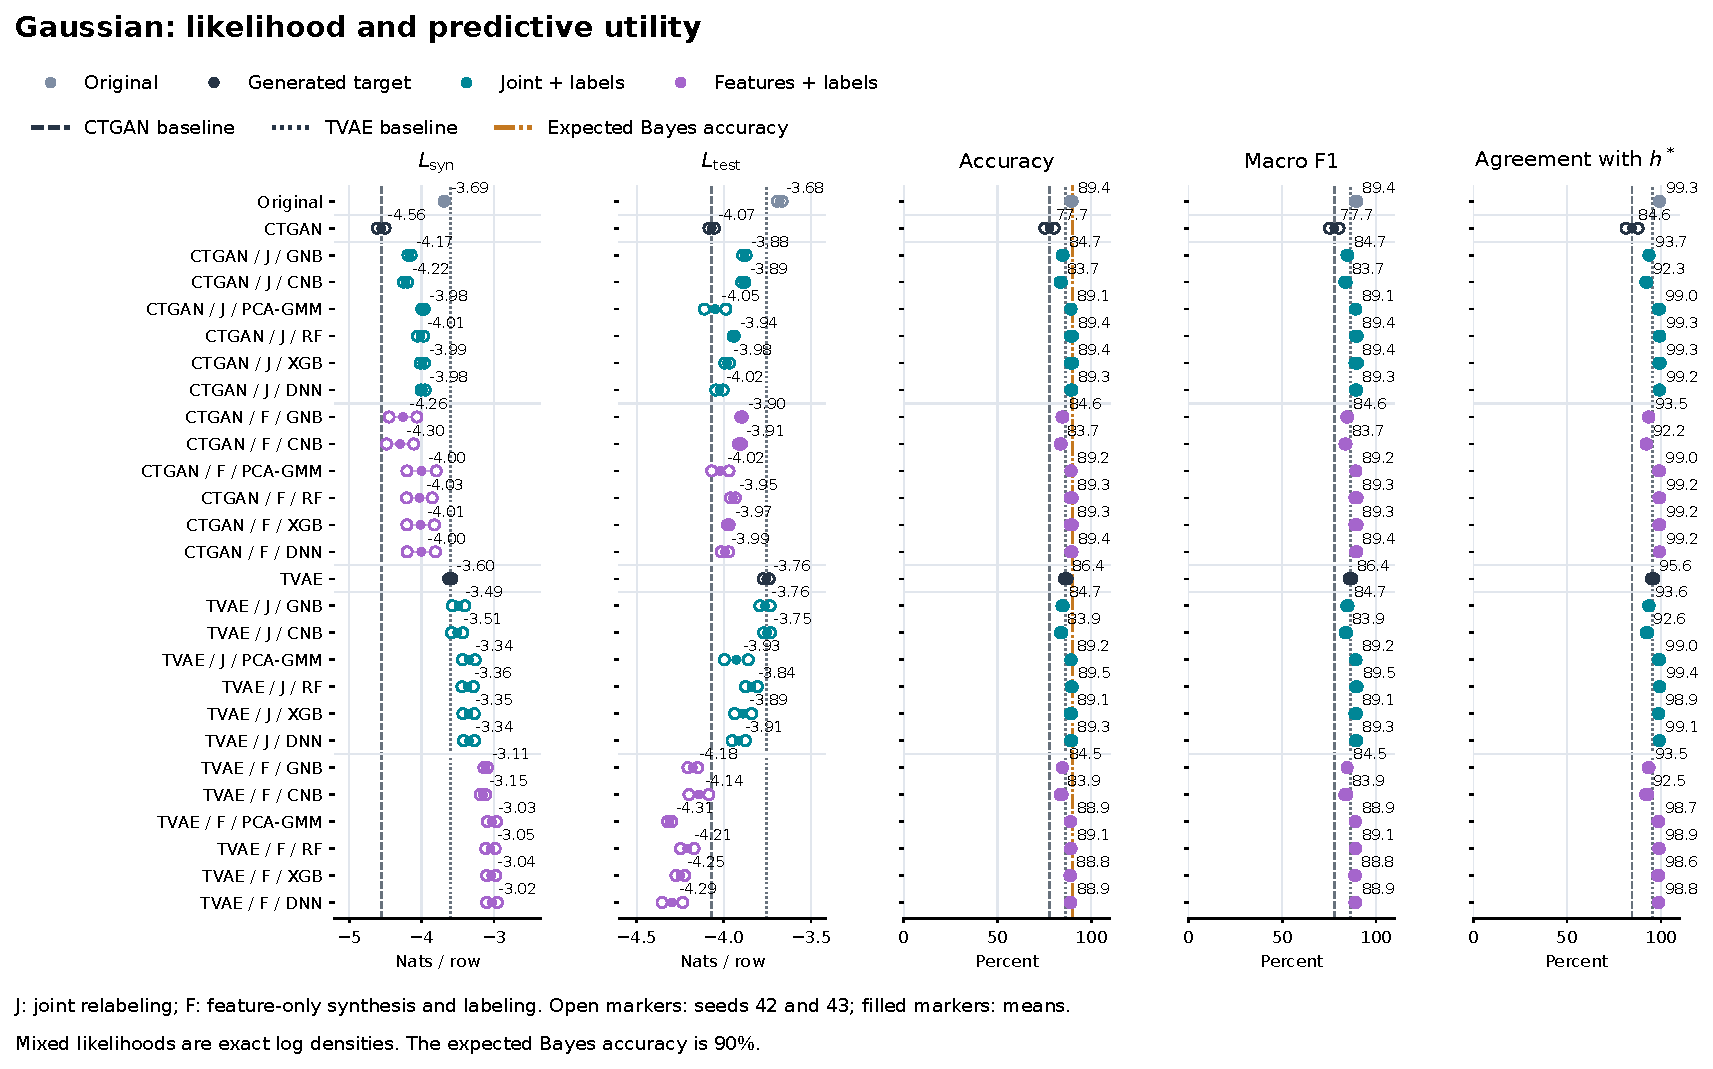
\includegraphics[width=\linewidth]{figures/gaussian.pdf}
\caption{Gaussian: all methods and both seeds. Likelihood panels and prediction panels use the definitions in Section 4.}
\label{fig:gaussian}\end{figure}
\end{landscape}\pdfpageattr{}
\begin{landscape}\pdfpageattr{/Rotate 90}
\begin{figure}[H]\centering
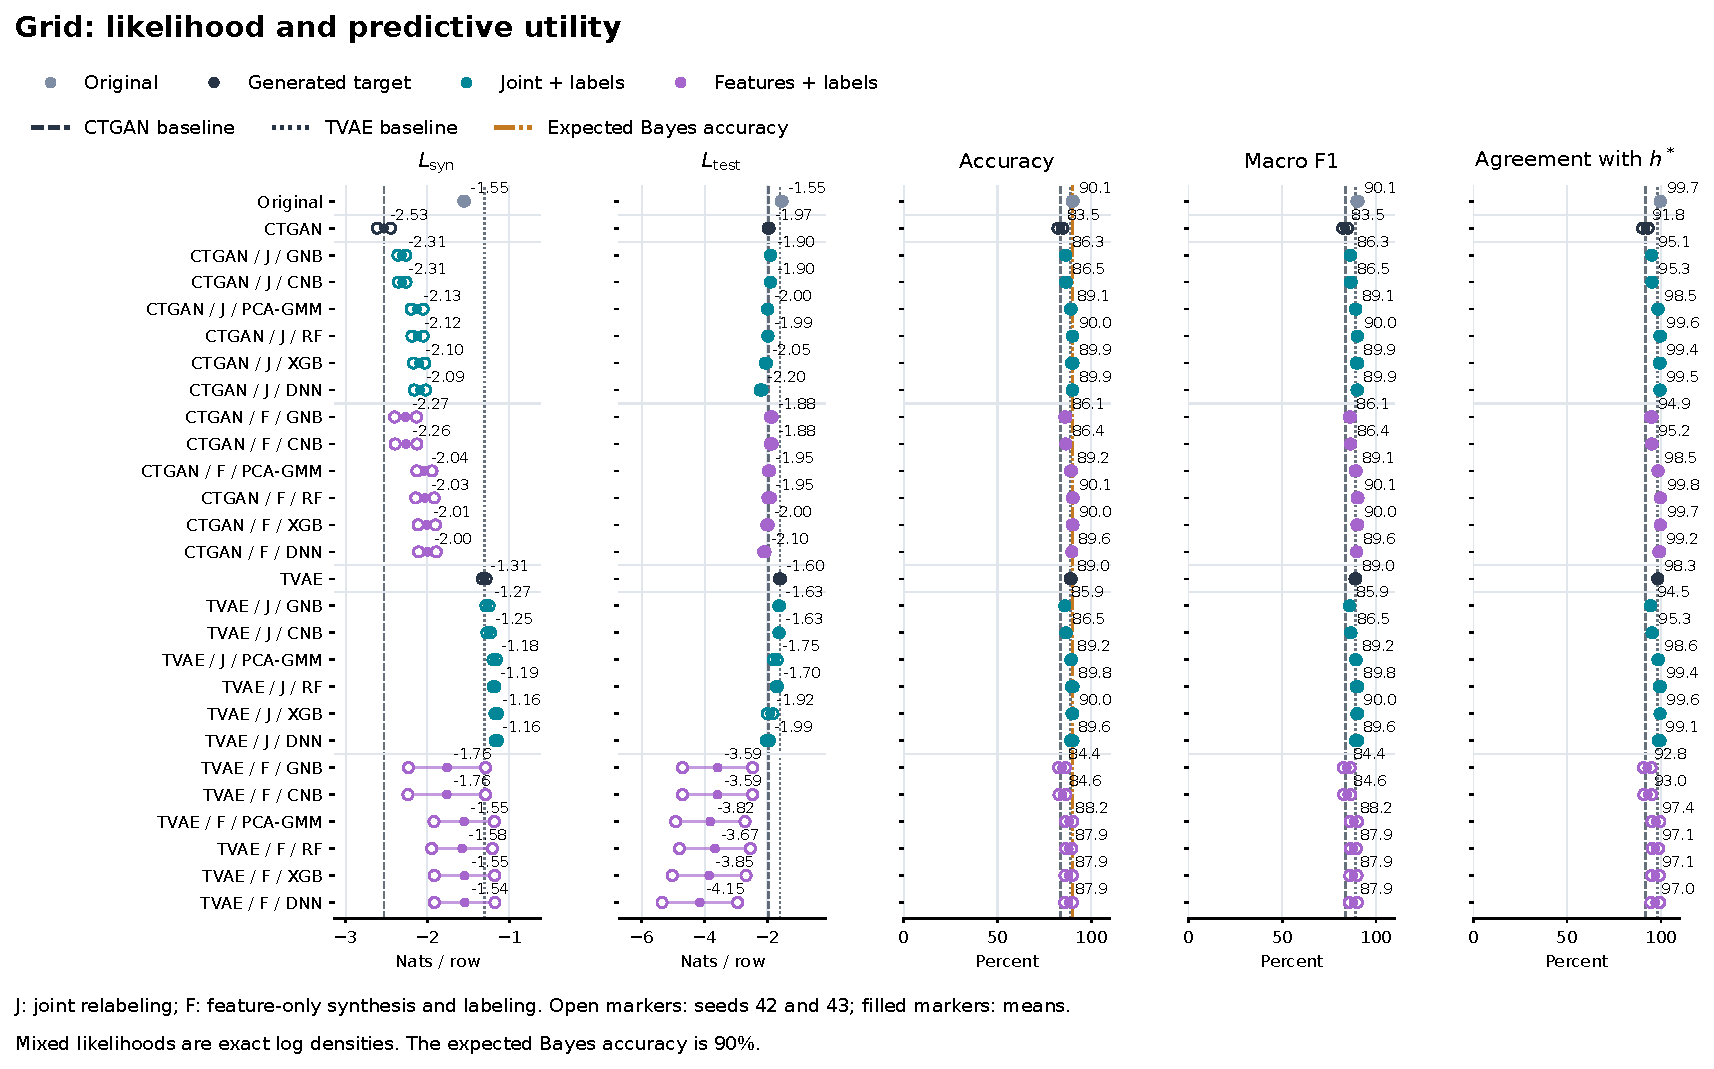
\includegraphics[width=\linewidth]{figures/grid.pdf}
\caption{Grid: all methods and both seeds. Likelihood panels and prediction panels use the definitions in Section 4.}
\label{fig:grid}\end{figure}
\end{landscape}\pdfpageattr{}
\begin{landscape}\pdfpageattr{/Rotate 90}
\begin{figure}[H]\centering
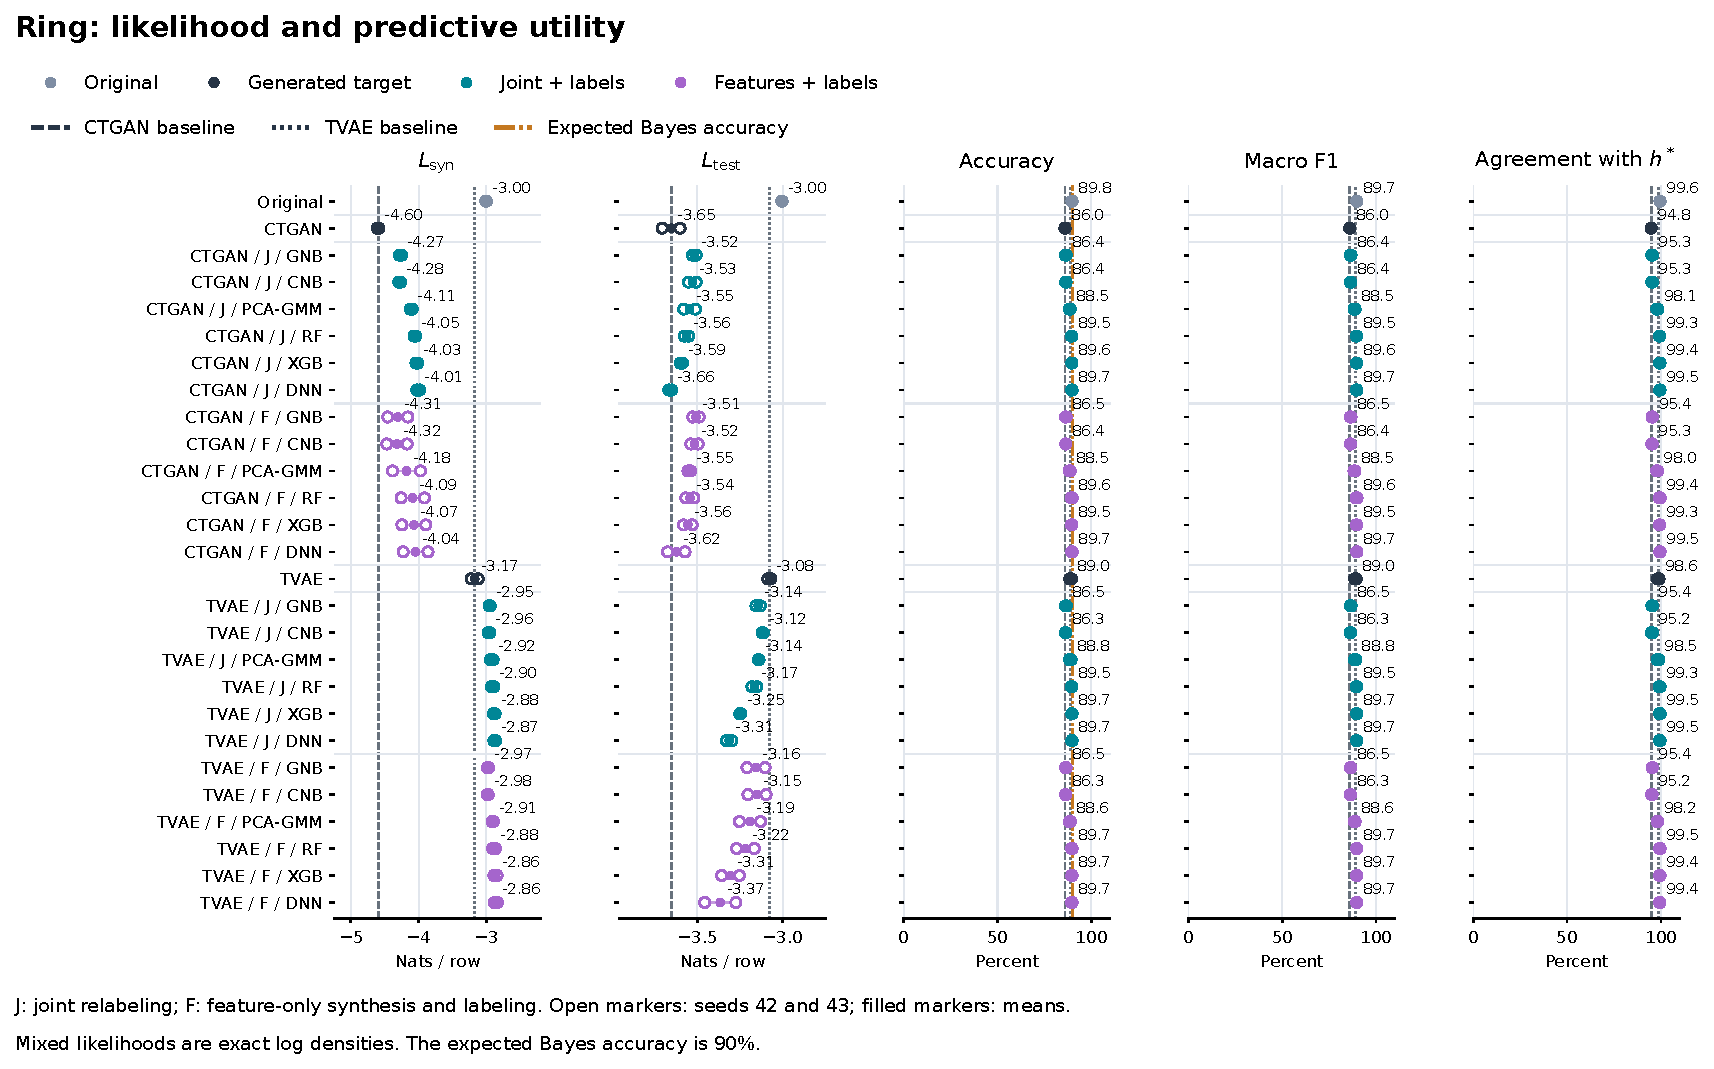
\includegraphics[width=\linewidth]{figures/ring.pdf}
\caption{Ring: all methods and both seeds. Likelihood panels and prediction panels use the definitions in Section 4.}
\label{fig:ring}\end{figure}
\end{landscape}\pdfpageattr{}
\begin{landscape}\pdfpageattr{/Rotate 90}
\begin{figure}[H]\centering
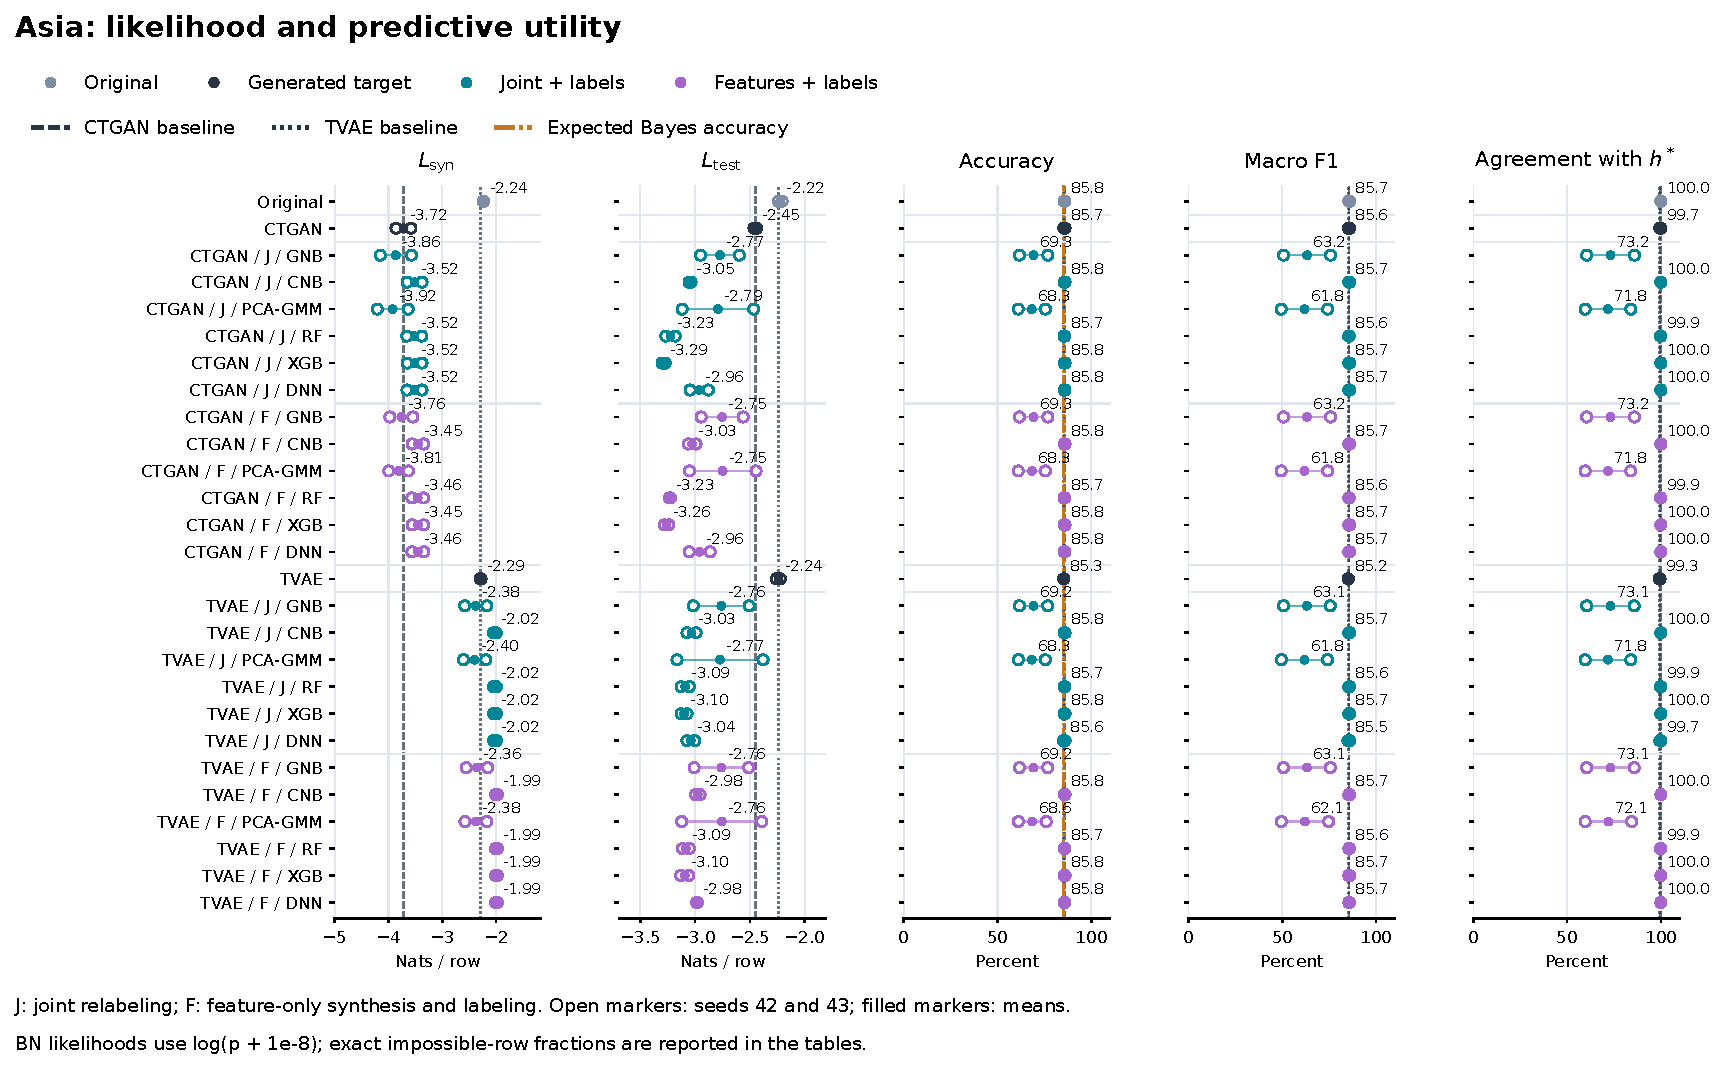
\includegraphics[width=\linewidth]{figures/asia.pdf}
\caption{Asia: all methods and both seeds. Likelihood panels and prediction panels use the definitions in Section 4.}
\label{fig:asia}\end{figure}
\end{landscape}\pdfpageattr{}
\begin{landscape}\pdfpageattr{/Rotate 90}
\begin{figure}[H]\centering
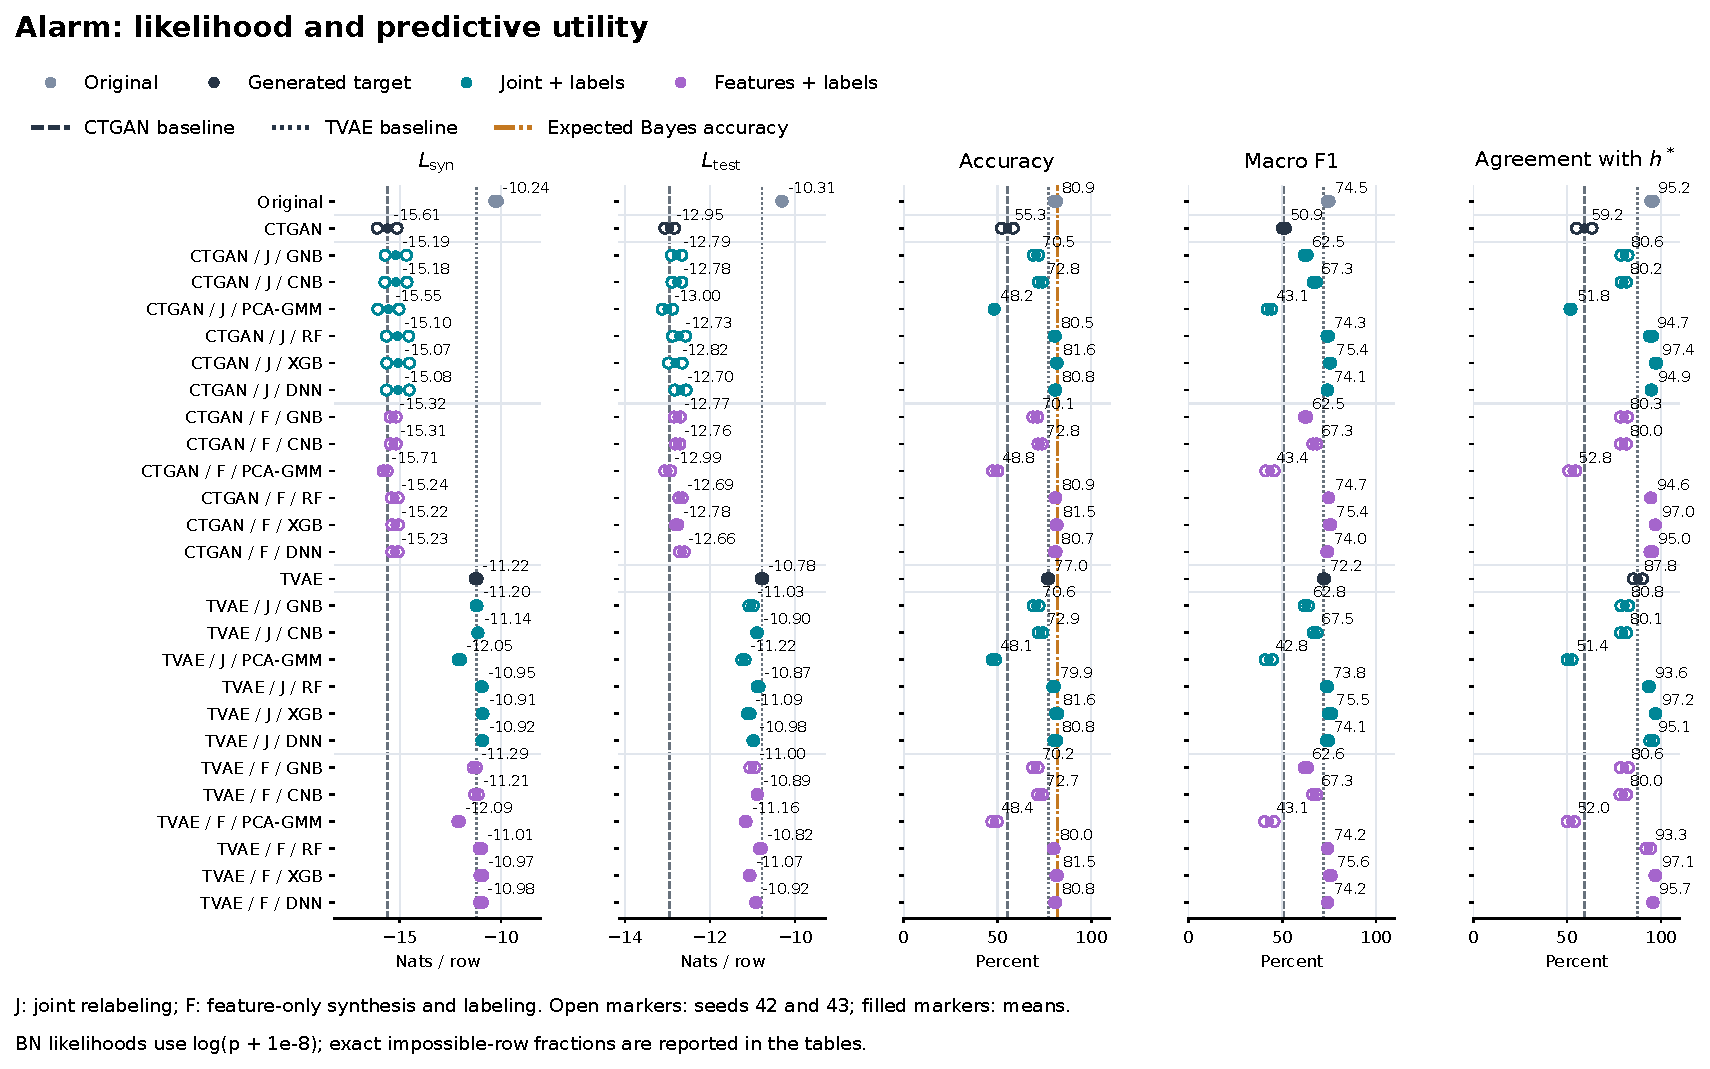
\includegraphics[width=\linewidth]{figures/alarm.pdf}
\caption{Alarm: all methods and both seeds. Likelihood panels and prediction panels use the definitions in Section 4.}
\label{fig:alarm}\end{figure}
\end{landscape}\pdfpageattr{}
\begin{landscape}\pdfpageattr{/Rotate 90}
\begin{figure}[H]\centering
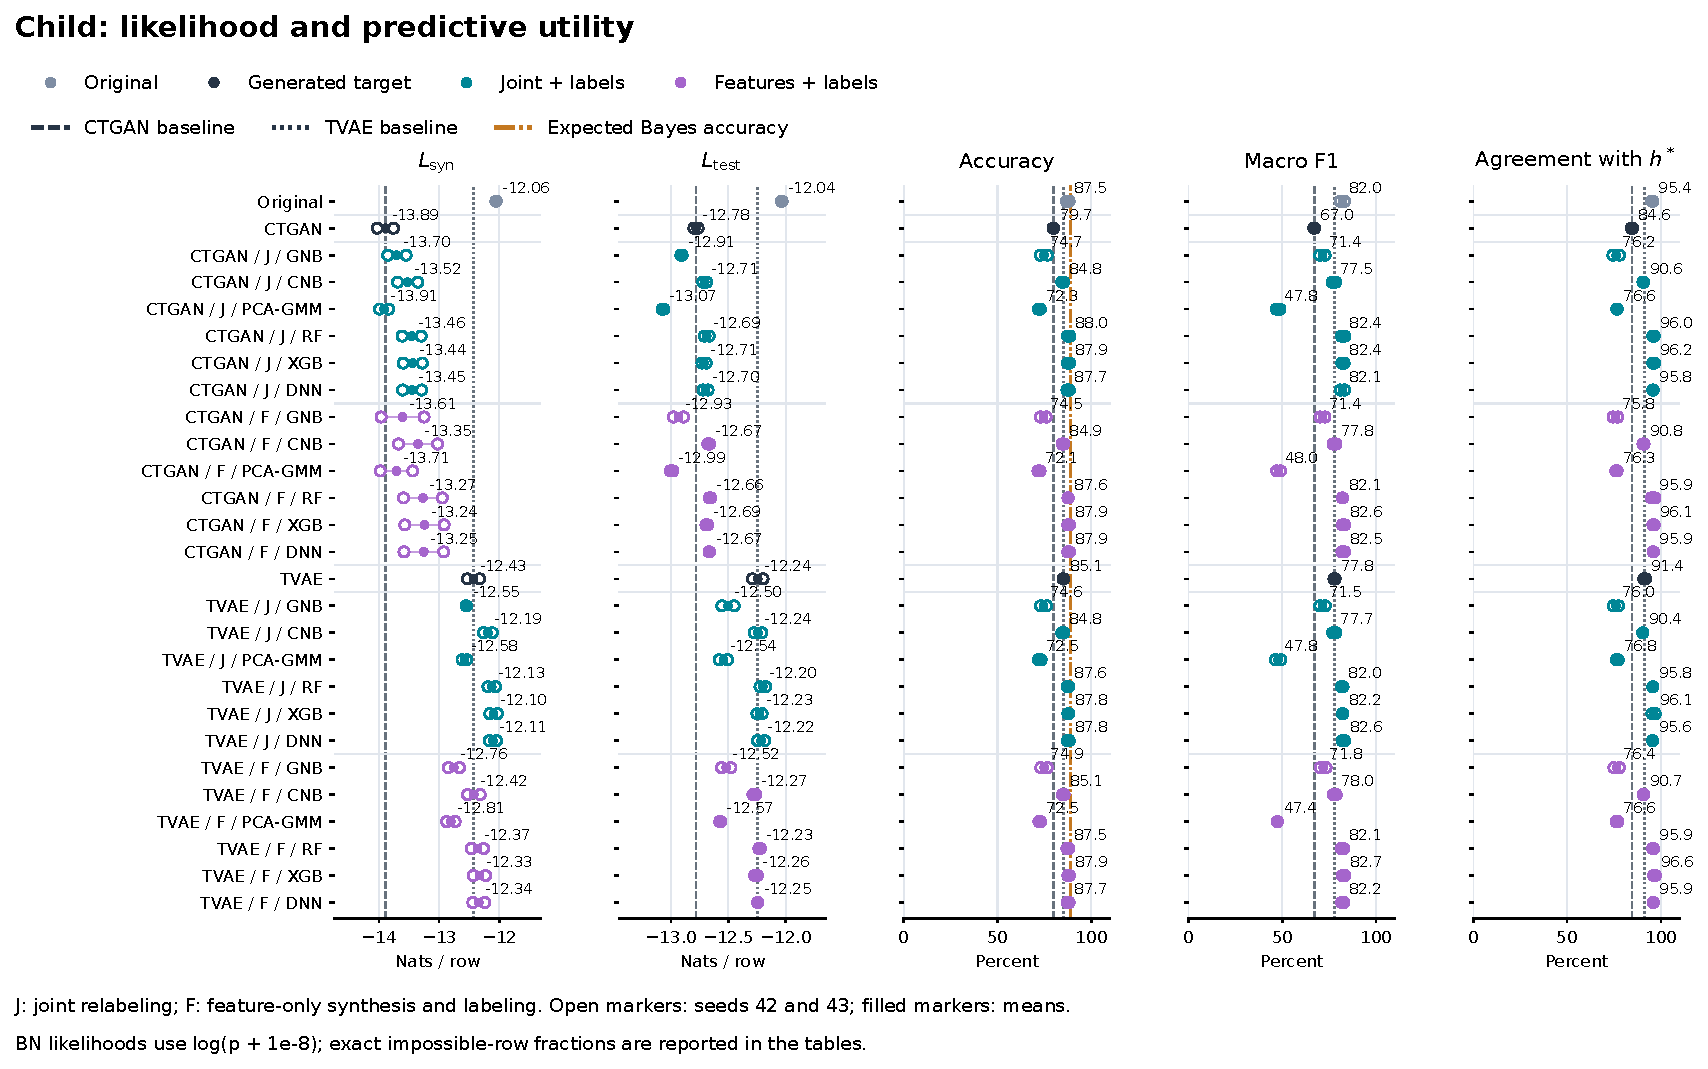
\includegraphics[width=\linewidth]{figures/child.pdf}
\caption{Child: all methods and both seeds. Likelihood panels and prediction panels use the definitions in Section 4.}
\label{fig:child}\end{figure}
\end{landscape}\pdfpageattr{}
\begin{landscape}\pdfpageattr{/Rotate 90}
\begin{figure}[H]\centering
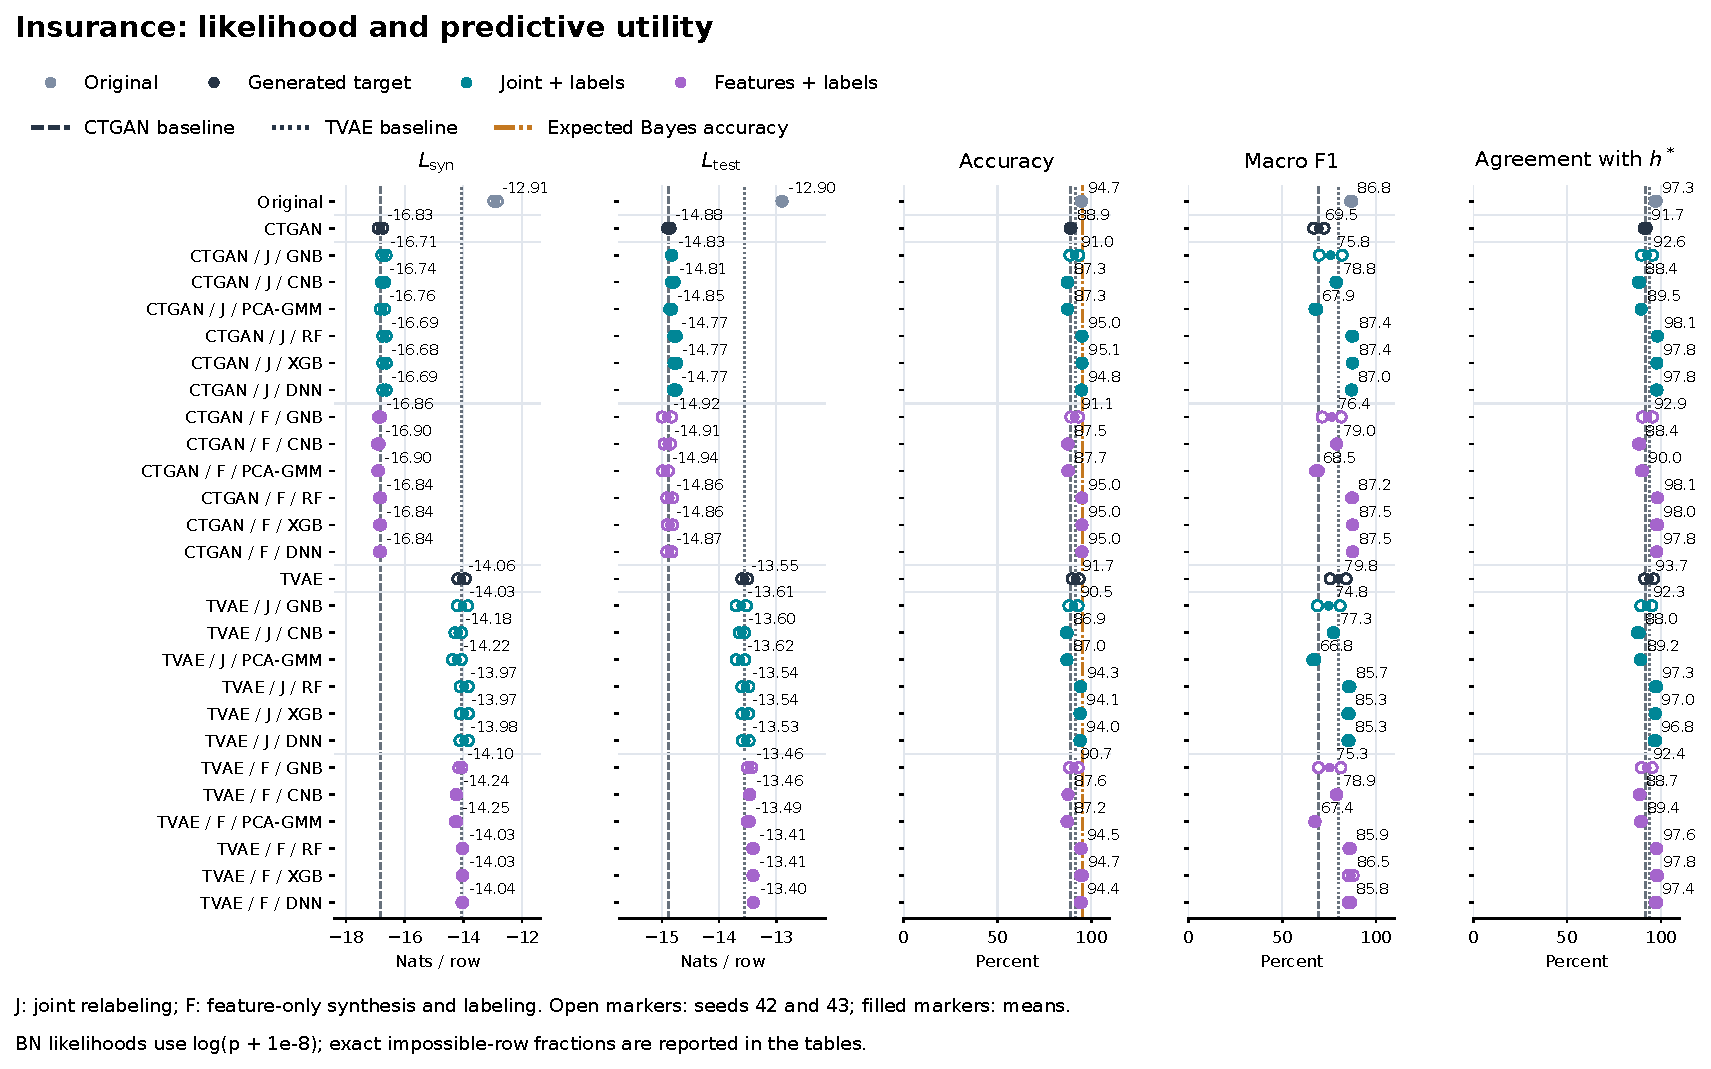
\includegraphics[width=\linewidth]{figures/insurance.pdf}
\caption{Insurance: all methods and both seeds. Likelihood panels and prediction panels use the definitions in Section 4.}
\label{fig:insurance}\end{figure}
\end{landscape}\pdfpageattr{}
\end{document}
